\documentclass[conference]{IEEEtran}

\usepackage[T1]{fontenc}
\usepackage{cite}
\usepackage{graphicx}
\usepackage{url}

\title{Cloud Architecture for an Epoch-Based Anonymous Event Relay}

\author{
\IEEEauthorblockN{Kevin Jin, John Yun}
\IEEEauthorblockA{Department of Computer Science\\
}
}

\begin{document}

\maketitle

\section{Problem \& Motivation}

\subsection{System and Workload}

This project studies the cloud architecture required to operate a dynamically sharded Riposte-style anonymous write relay. In the target model, clients submit encrypted messages into a shared epoch-batched database, and servers publish the resulting batch after the epoch completes. The server-side system is not intended to interpret application-level message semantics. Its responsibility is to admit writes, route them to shards, batch them, publish epoch results, and preserve enough availability and scalability for many clients to use the relay concurrently.

The workload is latency-tolerant and event-driven. Clients generate many independent write events, and the system batches those events into fixed epochs rather than trying to expose every write immediately. This model is a natural fit for applications where privacy is more important than sub-second interaction latency. Epoch batching increases anonymity by mixing many clients' activity into a common publication interval, but it also introduces a clear architectural trade-off: lower metadata exposure and better batch efficiency come at the cost of delayed visibility.

\subsection{Motivation}

The motivation follows directly from the threat model of anonymous communication systems such as Riposte. Corrigan-Gibbs, Boneh, and Mazi\`eres argue that hiding message contents is not sufficient when communication metadata can itself reveal sensitive relationships and behavior~\cite{riposte}. A server that observes who writes, when they write, which logical location they update, or which records they later read can infer communication patterns even if every payload is encrypted. This concern is central to anonymous messaging systems, where write location and timing metadata can undermine the anonymity set.

Modern analysis capabilities make this metadata problem more severe. Large-scale logs that once required manual investigation can now be clustered, summarized, and correlated using increasingly capable machine-learning and AI-assisted analysis tools. In a centralized platform, this creates a panopticon-like setting: users may not reveal message contents, but the operator can still infer communication frequency, timing patterns, and repeated associations from access patterns. The system studied here is motivated by reducing that observability while preserving a deployable anonymous write service.

\subsection{Cloud Deployment Rationale}

Although the long-term privacy vision can support decentralized operation, this prototype uses centralized cloud infrastructure to make measurement, debugging, and failure injection tractable. Centralization in the prototype does not mean the cloud operator is assumed to be fully trusted with message semantics or write metadata. Instead, the design goal is that the cloud-hosted servers should be able to operate a scalable anonymous write relay. A later deployment could decentralize shard operation by allowing independent parties to host shard replicas, including third-party leaders or followers in each leader-follower pair. That direction would move the trust model closer to the multi-operator assumptions common in anonymous communication systems while preserving the same epoch-batched interface.

Cloud infrastructure is appropriate for this stage because it exposes the operational constraints that determine whether a privacy-preserving design is deployable. It provides a controlled environment for repeatable experiments while still forcing the system to confront realistic bottlenecks in compute, bandwidth, availability, and managed state.

\subsection{Key Architectural Challenges}

\paragraph{Scalability}
The system must scale write admission and epoch publication as the number of clients grows. Cryptographic write protocols add server-side work, and larger anonymity sets produce larger epoch batches. Sharding can increase aggregate write capacity, but it also introduces routing, result publication, and coordination complexity.

\paragraph{Elasticity}
The system cannot safely change topology at arbitrary times. Scaling decisions are most natural between epochs because an active epoch depends on a consistent mapping from logical rows to shard-local storage. Changing shard membership mid-epoch could make routing and result interpretation inconsistent. It would also weaken the privacy model: each shard's epoch batch acts as an anonymity set for the writes routed there, so adding a new shard during the epoch can split traffic into smaller groups and leave some writes with a much smaller anonymity set.

\paragraph{Availability}
The coordinator and control plane must remain available enough to start epochs, close epochs, and publish results. A coordinator failure can block epoch progress, while shard failures can reduce write admission or prevent publication for part of the logical table. The architecture therefore has to distinguish process health, control-plane authority, and shard-level availability.

\paragraph{Cost}
Privacy-preserving protocols can increase compute, bandwidth, and storage costs compared with a conventional centralized message relay. Batching, sharding, and managed control state improve deployability, but each also introduces resource overhead that must be justified by the privacy benefit.

\paragraph{Security}
Encrypted message contents are not enough if metadata remains visible. The architecture must define trust boundaries among clients, the cloud operator, server operators, and possible future third-party shard operators. The system goal is to reduce what infrastructure can infer from write location, timing, and routing metadata, while still preserving enough operational visibility to debug and evaluate the deployment.

These challenges are architectural rather than purely cryptographic. The cryptographic protocol motivates what the server should not learn, but the cloud design determines whether the system can admit enough writes, recover from failures, and remain affordable under realistic load. The rest of the report evaluates that architecture while keeping the implementation-specific topology, failure experiments, cost estimates, and measured performance separate from this motivation.

\section{Related Work}

\subsection{Riposte}

Riposte is the closest technical and conceptual baseline for this project. It provides an anonymous messaging protocol in which clients write into a shared database without revealing the sender or write location to any single honest server~\cite{riposte}. Its design uses epochs to batch many messages, which improves anonymity by allowing each user's write to be hidden within a larger population. Riposte also addresses malicious clients, whose malformed writes could otherwise corrupt shared state. The main trade-off is that the system is designed for latency-tolerant workloads: users gain stronger metadata protection by accepting delayed publication and additional server-side work.

This project does not propose a new anonymous-write protocol. Instead, it asks what cloud architecture is needed to operate a Riposte-style event relay under realistic deployment constraints. The implementation therefore emphasizes sharding, epoch coordination, coordinator availability, shared control state, and scaling evaluation. In that sense, Riposte supplies the privacy-preserving write abstraction, while this project studies how that abstraction interacts with cloud elasticity, failure domains, and operational cost.

\subsection{Private Information Retrieval}

Private Information Retrieval (PIR) protects read access patterns by allowing a client to retrieve database information without revealing which record was requested. Corrigan-Gibbs et al. improve the practicality of PIR by compressing queries and amortizing server computation across repeated operations~\cite{pircompressed}. This line of work is relevant because a complete private communication system must protect both writes and reads. Riposte-style anonymous writes could be paired with PIR so users can access remote message or bulletin-board state without revealing which records they read. Even if message contents are encrypted, a platform that knows who communicates with whom can infer sensitive associations. Combining anonymous writes with private reads therefore has an ethical benefit beyond technical confidentiality: it reduces metadata exposure and weakens the power imbalance between users and platform operators.

PIR also illustrates the architectural cost of privacy. Protecting access patterns can increase server computation, communication, and batching complexity. Those costs make cloud evaluation important: a protocol that is asymptotically efficient may still be difficult to operate if managed infrastructure, network bandwidth, or CPU utilization become bottlenecks. The current prototype focuses more directly on anonymous write admission and epoch publication, but PIR motivates the broader requirement that a privacy-preserving platform must eventually handle both sides of the interaction.

\subsection{Anysphere}

Anysphere is a metadata-private communication system that emphasizes practical deployment rather than only protocol design~\cite{anysphere}. Its whitepaper makes the same core observation that motivates this project: end-to-end encryption protects message contents, but it does not hide who communicates with whom, how often, or when. Anysphere addresses this by combining authenticated encryption, fixed-rate client sending, and PIR-based retrieval from user outboxes. In its threat model, servers and network observers should not learn communication patterns even if server infrastructure is compromised.

Anysphere is useful as a practical comparison point because it shows how metadata privacy changes system architecture. Users send cover traffic when they do not have real messages, and receivers use PIR so the server cannot tell which outbox is being read. These choices improve privacy but introduce costs in bandwidth, client scheduling, server computation, and latency. This project makes a different design trade-off: it focuses on Riposte-style anonymous event submission and epoch-batched publication, then evaluates how cloud sharding, coordinator availability, and scaling mechanisms affect deployability. Both systems reinforce the same lesson: metadata privacy is not an optional feature layered on top of a conventional messaging service; it changes the storage, communication, and scaling model of the system.

\subsection{Verifiable Secret Sharing}

Verifiable Secret Sharing (VSS) addresses a different but related problem: how distributed participants can share and later reconstruct secret state while detecting incorrect behavior. The ``Verifiable Secret Sharing Simplified'' work improves VSS constructions for synchronous and asynchronous settings while preserving strong fault-tolerance properties~\cite{vsssimplified}. Its emphasis is not anonymous communication, but distributed correctness under partial trust.

That distinction is useful because anonymous systems still need mechanisms for trust and selective disclosure. A future system built on an anonymous relay may want to enforce threshold policies without revealing all underlying membership or credential state. VSS-style techniques suggest one way to reason about these policies: secret or membership-related state can be distributed so that no single server learns the sensitive relationship, while reconstruction or verification requires enough independent evidence.

\subsection{Ring Referral}

Ring Referral extends anonymity techniques to credential presentation. It lets a user prove possession of a credential issued by one member of an ad hoc ring without revealing which issuer produced it~\cite{ringreferral}. The scheme is publicly verifiable and supports privacy-preserving authentication, where the protected metadata is the relationship between issuer and user rather than the location of a database write.

This is relevant because anonymous systems may need more than anonymous transport alone. Users may want confidence that another participant has some credential, group membership, or endorsement, while still avoiding disclosure of exactly who vouched for them. Ring Referral offers a model for this kind of privacy-preserving trust: a user can prove that a credential came from an acceptable set without exposing the precise relationship. PIR protects read access patterns. Riposte protects anonymous write locations and sender metadata. Ring Referral protects credential provenance. Together, these systems show that privacy-preserving infrastructure must protect multiple metadata surfaces, not only encrypt payload contents.

\subsection{Synthesis}

Taken together, prior work shows that privacy-preserving communication is feasible but operationally expensive. Cryptographic systems define the privacy properties, while architecture determines whether those properties can be delivered with acceptable throughput, availability, elasticity, and cost. This report therefore treats the cloud deployment not as an implementation detail, but as part of the privacy system's viability.

\section{System Architecture}

\subsection{Design Goals and Constraints}

The architecture is designed around five goals:
\begin{enumerate}
\item Preserve metadata privacy by preventing server components from needing to interpret message semantics beyond the anonymous write protocol.
\item Preserve epoch consistency so all writes accepted for an epoch are interpreted against a stable shard topology and published as part of that epoch's result.
\item Scale the write path horizontally by distributing logical rows across shards.
\item Keep the control plane available without allowing split-brain control decisions.
\item Remain deployable on cloud infrastructure so performance and failure behavior can be measured under realistic operational constraints.
\end{enumerate}

The main constraints follow from those goals. The current Riposte-style upload path is a three-step client/server exchange: \texttt{Upload1} creates a session, \texttt{Upload2} returns the server challenge, and \texttt{Upload3} completes validation. A queue-first, fire-and-forget design is possible, but it would require redesigning how session allocation, challenge generation, and proof validation become durable before the client receives a final acceptance signal. This implementation therefore places the durable ingestion boundary after a shard has accepted a completed \texttt{Upload3}. The current design also keeps topology changes at epoch boundaries, because changing shard membership during an epoch would make row routing, result interpretation, and anonymity-set reasoning ambiguous. Full replay of partial shard-side \texttt{Upload1}/\texttt{Upload2} state after shard death and exact idempotence for redelivery after commit-but-before-queue-delete remain protocol-hardening limitations.

\subsection{Deployment Architecture}

Figure~\ref{fig:deployment-architecture} summarizes the deployment view. The write path and read path use different ingress layers because their protocols are different. Writes use a Network Load Balancer with the existing custom TCP/TLS RPC protocol, so the load balancer is connection-oriented and forwards client upload traffic to coordinator processes. Reads use an Application Load Balancer with HTTP JSON requests, so the load balancer can make request-aware routing and semantic health-check decisions. In the multi-coordinator configuration, the NLB distributes upload RPCs across coordinator processes. All coordinators can serve data-plane upload routing when the shared control store reports an active accepting epoch, but only the coordinator holding the fenced lease is authoritative for control-plane mutations such as starting epochs, completing epochs, or applying topology changes.

\begin{figure*}[!t]
\centering
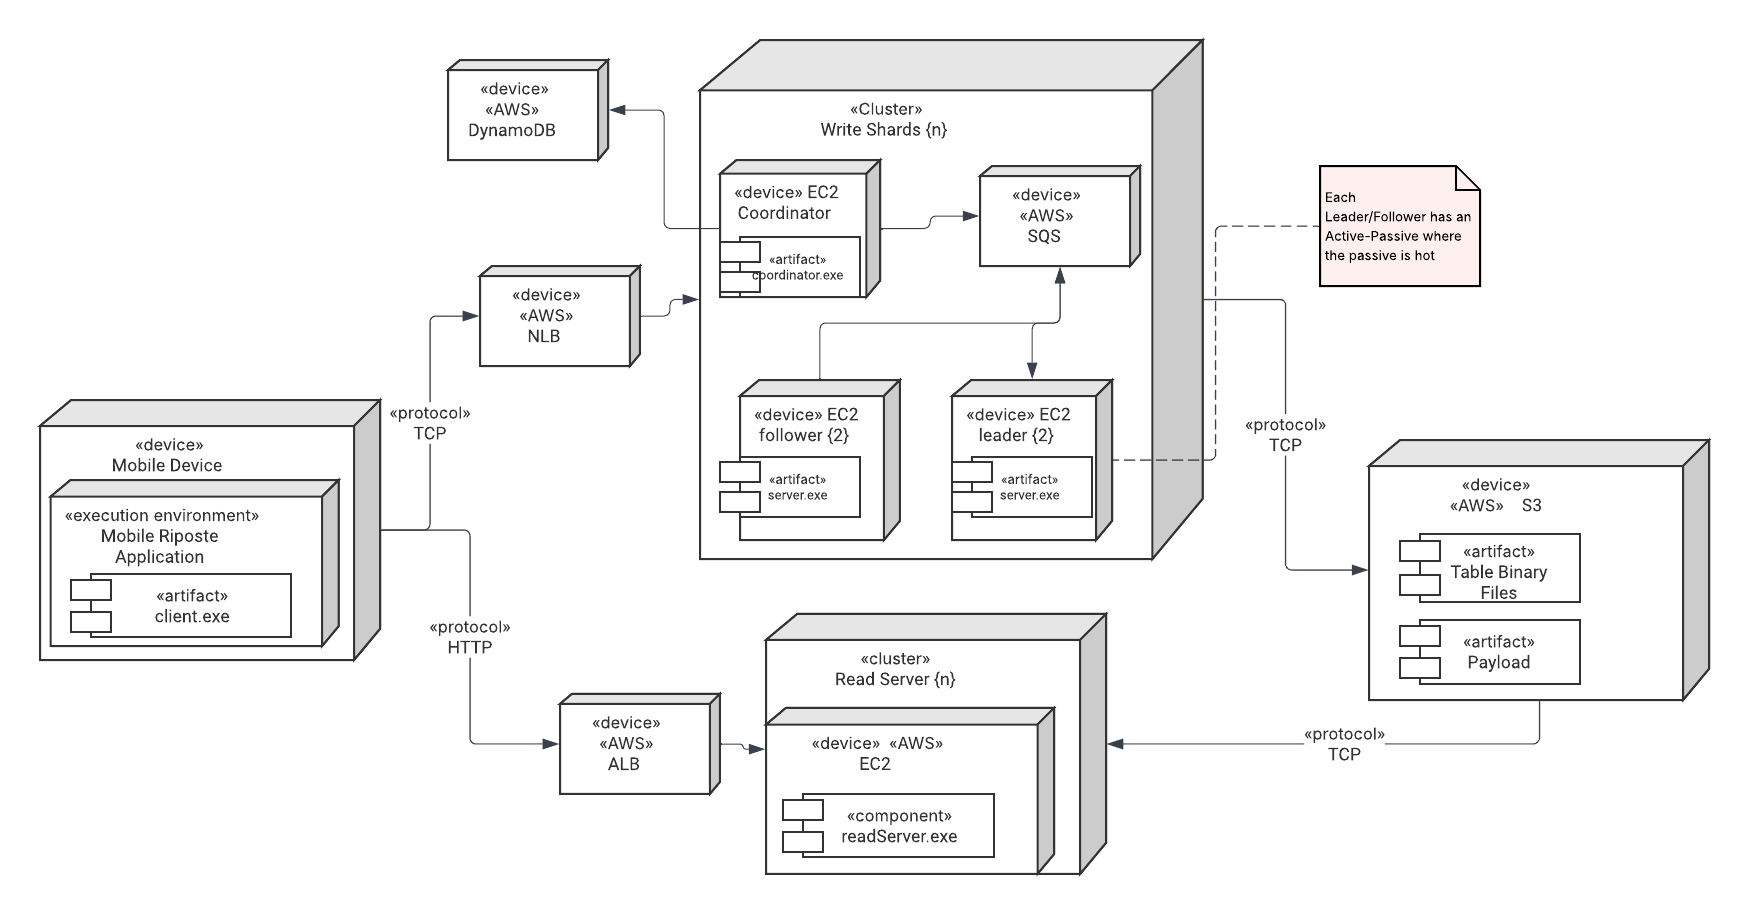
\includegraphics[width=\textwidth]{figures/deployment-diagram.png}
\caption{Deployment architecture for the cloud-hosted dynamically sharded Riposte prototype. Writes use NLB-backed custom TCP/TLS RPC to coordinator processes, while reads use ALB-backed HTTP JSON requests to stateless read servers. Coordinators and shard servers run on EC2, DynamoDB stores control state, SQS dispatches shard-local completed-upload work, and S3 stores published table artifacts and completed-upload payloads.}
\label{fig:deployment-architecture}
\end{figure*}

The persistent control plane is backed by DynamoDB. It stores coordinator lease state, epoch metadata, shard topology, in-flight coordinator sessions, scaling recommendations, and epoch-cycle milestones. Shard servers are deployed as leader/follower pairs. Each shard owns a contiguous range of global rows and processes a fixed local table. After a shard leader accepts a completed upload, it writes the completed-upload payload to S3 and sends pointer messages to the shard ingestion queues. Shard workers consume queue messages, load payloads from S3, process the upload, and delete the SQS message only after successful processing. Result artifacts are published per shard at epoch completion.

\subsection{Component Architecture}

Figure~\ref{fig:component-architecture} shows the major runtime components. The client implements the upload protocol and treats the coordinator tier as the routing entry point. Each coordinator can route uploads to the correct shard, rewrite global rows to shard-local coordinates, use shared coordinator session records, monitor shard health, and expose status/admin RPCs. Control and topology mutations are guarded by the coordinator lease so that only one coordinator acts as the authoritative writer.

\begin{figure*}[!t]
\centering
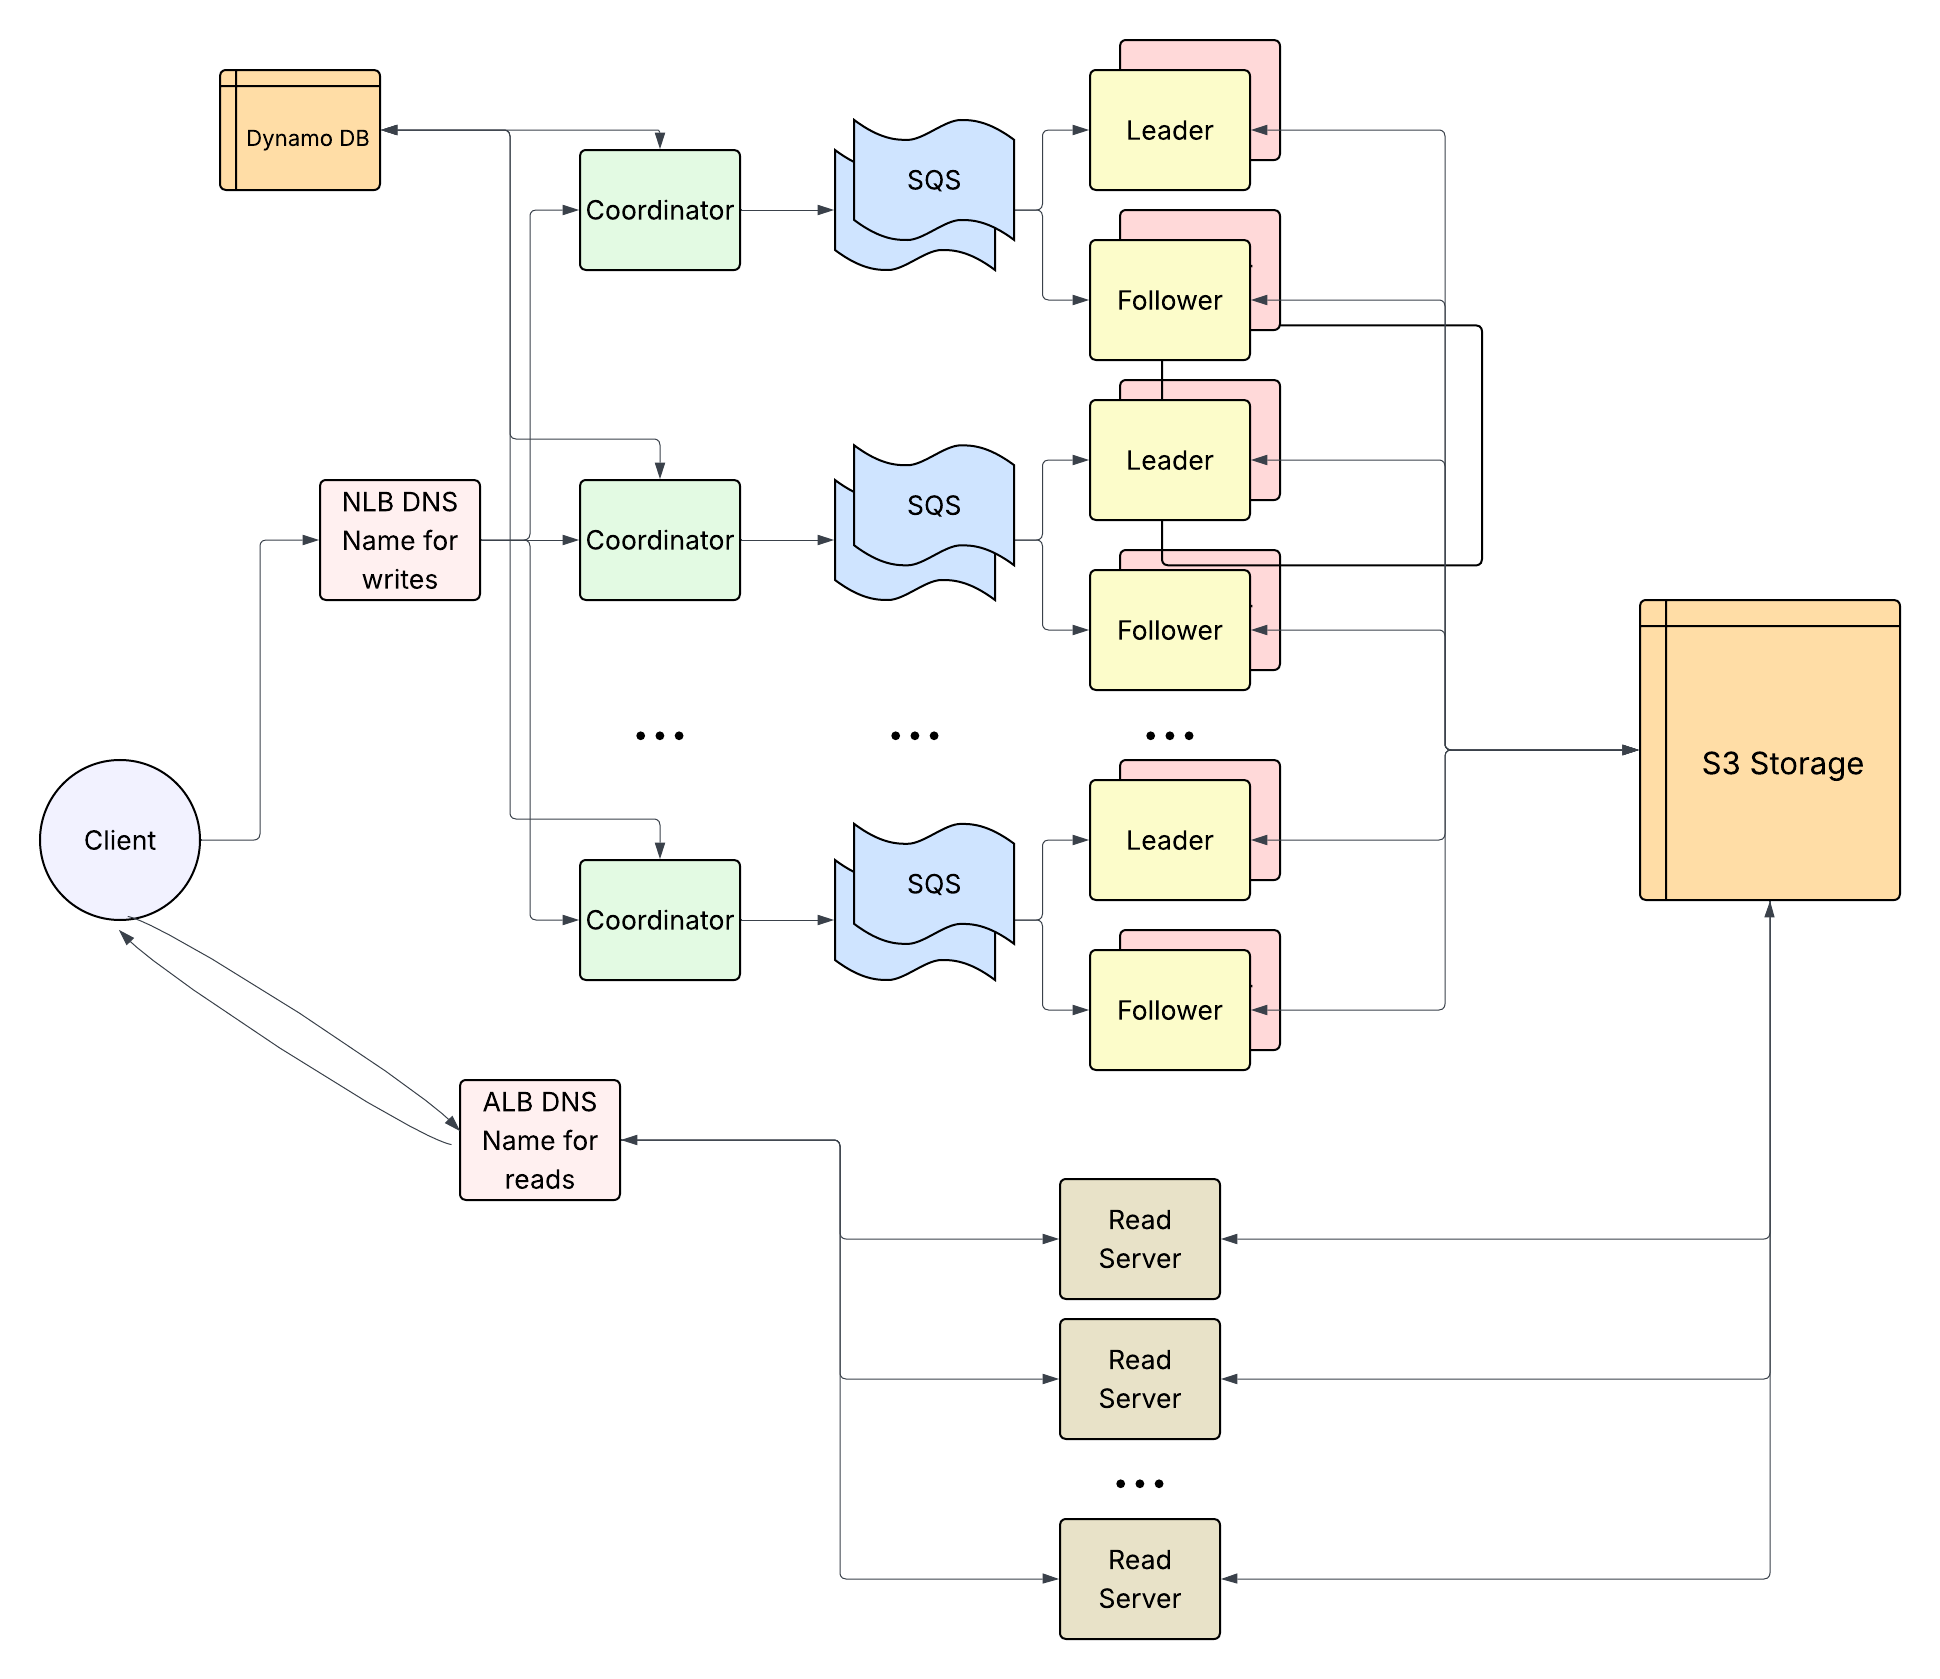
\includegraphics[width=0.95\textwidth]{figures/component-diagram.png}
\caption{Component architecture for the dynamically sharded Riposte deployment. Write traffic enters through the NLB DNS name and coordinator tier, shared control/session state is stored in DynamoDB, shard-local completed-upload work is dispatched through SQS, payload and table artifacts are stored in S3, and stateless read servers serve S3-published tables through the ALB DNS name.}
\label{fig:component-architecture}
\end{figure*}

The control store and session store separate process-local coordinator state from shared authority. DynamoDB-backed sessions allow a different coordinator process to continue \texttt{Upload2} or \texttt{Upload3} after \texttt{Upload1} was routed elsewhere. Coordinators that do not hold the lease are non-authoritative for control mutations, but they can still route upload traffic using shared epoch, topology, and session state. The autoscaler reads completed-epoch recommendations and participates in the epoch-cycle state machine for applying topology changes. Before the current shard configuration changes, the control plane re-checks epoch safety, shard inventory, and coordinator authority so that scaling is applied only between epochs.

Within each shard, the leader remains responsible for interactive upload validation. The S3/SQS ingestion boundary starts only after that validation succeeds at \texttt{Upload3}. This split preserves the protocol's interactive checks while making the expensive post-acceptance processing durable and replayable. The worker side of the shard processes queued completed uploads and feeds the epoch result pipeline.

\subsection{Write and Epoch Interaction Flow}

Figure~\ref{fig:write-epoch-interaction} describes the main interaction flow. A client first calls \texttt{Upload1}. The coordinator checks that the shared control store reports an active accepting epoch, selects the owning shard by global row, rewrites the row to shard-local coordinates, allocates a global session identifier, persists the session, and forwards the request to the shard. The client then completes \texttt{Upload2} and \texttt{Upload3}; if a later phase reaches a different coordinator, that coordinator can recover the session from the shared session store and continue routing.

\begin{figure*}[!t]
\centering
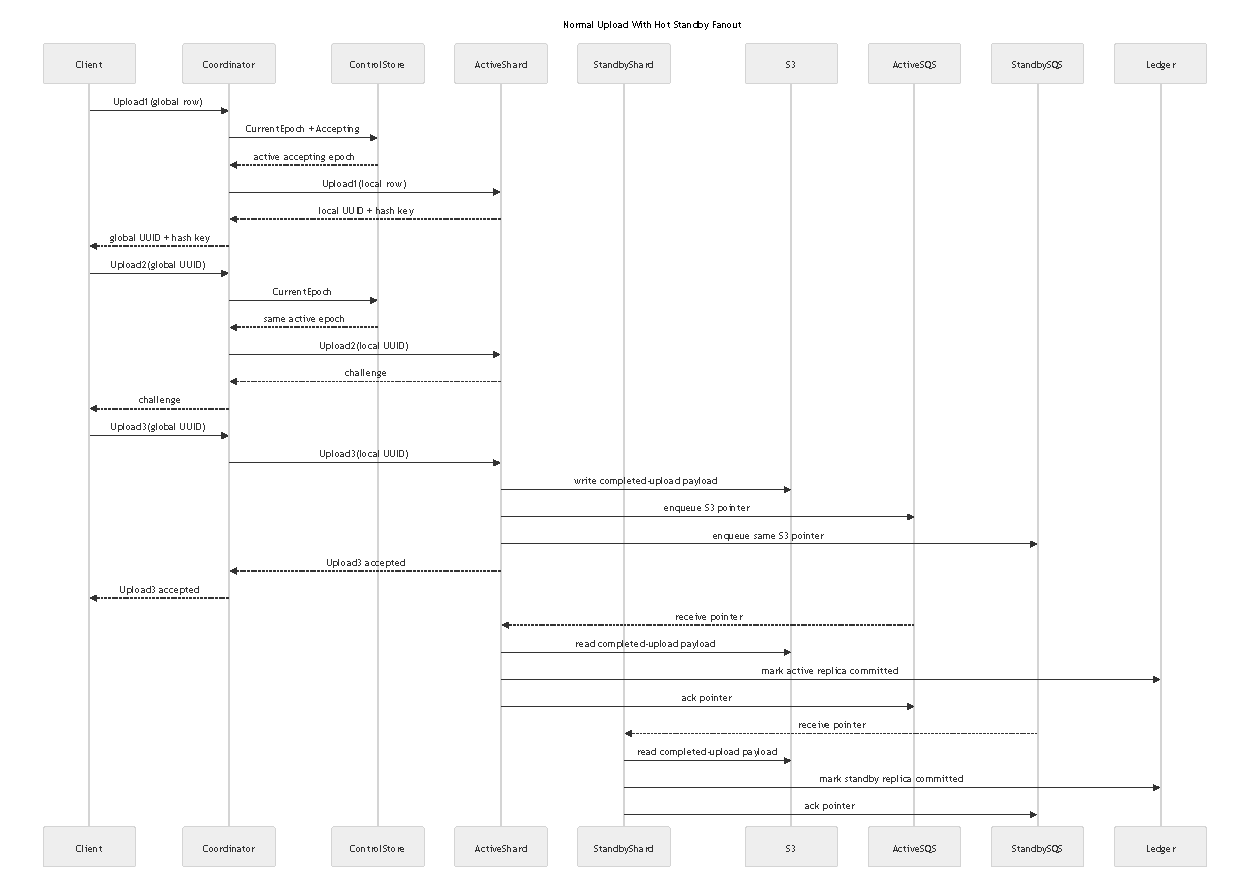
\includegraphics[width=\textwidth]{figures/normal-upload-hot-standby.pdf}
\caption{Normal upload interaction with hot-standby coordinator routing. The flow shows client upload phases, shared coordinator/session state, shard forwarding, durable post-\texttt{Upload3} ingestion, and the standby path that can continue routing through shared state.}
\label{fig:write-epoch-interaction}
\end{figure*}

After the shard accepts \texttt{Upload3}, the durable ingestion boundary begins. The shard leader writes the full completed-upload payload to S3, sends SQS pointer messages to the shard ingestion path, and returns success only after those durable writes succeed. A worker receives an SQS pointer, reads the payload from S3, runs prepare/commit processing, and acknowledges the SQS message only after processing succeeds. This means post-\texttt{Upload3} work can be retried after worker failure or process restart, while preserving the distinction between interactive validation and durable background processing.

At epoch completion, each shard publishes its result for its global row range. The coordinator records completed-epoch scaling metrics and persists a scaling recommendation. The epoch-cycle and autoscaler path described above then determines whether that recommendation becomes the next epoch's authoritative shard configuration.

\subsection{Scaling Model}

The logical table grows by adding shards. Each shard contributes \texttt{db.TABLE\_HEIGHT} logical rows, currently 256 rows. A one-shard deployment therefore exposes 256 global rows, while a two-shard deployment exposes 512 global rows. The coordinator treats the shard map as the authoritative mapping from global rows to shard-local rows. For example, global row 256 maps to local row 0 on shard 1 when shard 0 owns rows [0,256) and shard 1 owns rows [256,512).

Scaling recommendations are computed from accepted-request density after an epoch completes. The density is the accepted upload count divided by the logical row count. Growth, shrink, or keep decisions are proposals only until applied between epochs. This boundary is required for correctness and privacy. Correctness requires a stable row-to-shard mapping for the whole epoch, and privacy requires stable per-shard anonymity sets. Client write rows are expected to be chosen uniformly at random across the active global row space; changing the shard map mid-epoch would split that random process across two different topologies. A newly activated shard could receive only a small suffix of the epoch's writes, while existing shards would have mixed pre-change and post-change traffic. That would shrink or skew the per-shard anonymity set and make result interpretation ambiguous. Applying a recommendation updates the current shard configuration but does not mutate historical epoch snapshots. The SQS/S3 ingestion boundary improves durability and replayability of accepted work, but it does not by itself provision new EC2 instances. Scale-out currently depends on cold spare shard endpoint inventory: spare shard processes are configured but not part of the active shard map until a recommendation activates them for a later epoch. This is distinct from the warm active-passive coordinator and shard-replica paths, where standby processes are already running for availability rather than capacity growth.

\subsection{Storage Strategy}

DynamoDB is the authoritative control and session store. The \texttt{lease} record stores the active coordinator holder, fencing token, and expiry. The \texttt{epoch} record stores current epoch metadata and whether writes are accepting. The \texttt{shard-config} record stores the current topology, while immutable \texttt{shard-config\#epoch\#<id>} records preserve historical topology for completed epochs. Session records identify routed uploads between \texttt{Upload1} and \texttt{Upload3}, and scaling records store completed-epoch recommendations. The \texttt{epoch-cycle} record exposes whether the system is active, waiting on a recommendation, has applied scaling, or skipped scaling.

S3 and SQS form the completed-upload ingestion layer. S3 stores the full completed-upload payload because the payload is larger and more durable than what should be carried directly in a queue message. SQS stores compact pointers to those payloads and provides redelivery when a worker fails before acknowledgement. When hot standby ingestion is enabled, each shard has separate active and standby queues, such as \texttt{shardN-active} and \texttt{shardN-standby}. The same completed-upload pointer is sent to both queues so the active and standby replicas can process the write independently and the standby remains caught up for promotion. Per-shard result files remain the epoch publication artifacts. S3 can also serve as the longer-term home for result and recovery artifacts, while SQS is specifically the live durable ingestion queue after \texttt{Upload3}.

\subsection{Failure Domains}

The architecture separates several failure domains. Coordinator process failure affects control operations such as starting epochs or applying topology changes if the failed process held the lease, but NLB routing and shared sessions allow another coordinator to continue data-plane upload routing when the epoch remains accepting. If a coordinator dies between upload phases, the client's next RPC can reach another coordinator, which recovers the session from DynamoDB and forwards the next phase to the same shard. If a coordinator dies during an in-flight RPC, the client may observe that RPC as failed and retry through the NLB. The shard does not independently contact the client; it replies through whichever coordinator forwarded the request. A stale coordinator cannot mutate control state because the lease and fencing token prevent old authority from being reused. DynamoDB availability affects shared control and session state, so it is a central dependency for coordinated operation.

Shard failures affect the shard's local row range. A leader failure can interrupt interactive upload validation for that shard, while worker failure after \texttt{Upload3} is mitigated by SQS redelivery and S3 payload persistence. S3 availability affects access to completed-upload payloads, and SQS availability affects worker dispatch. The NLB affects public coordinator ingress but does not own correctness. Client/load-generator failure affects submitted workload rather than stored control state. Autoscaler failure delays scaling application but does not prevent the current topology from continuing to serve an active epoch.

\subsection{Trust Boundaries}

Clients do not trust servers with message semantics beyond the anonymous write protocol. Payload contents remain opaque to the infrastructure, while servers provide routing, admission, storage, and publication services. The cloud operator and managed services are trusted for operational availability and integrity of infrastructure, but the architecture is designed so that they do not need plaintext message semantics to operate the system.

DynamoDB centralizes control authority and session recovery in the current cloud prototype. SQS and S3 become trusted durable ingestion infrastructure after upload acceptance. Shard leaders, followers, and workers are trusted to execute the server protocol for their assigned row ranges, but the long-term architecture can reduce single-operator trust by allowing independent parties to host shard replicas. IAM roles, TLS-protected RPC, security groups, and queue/bucket permissions enforce operational boundaries; the detailed configuration is discussed in the implementation section.

\section{Implementation Details}

\subsection{Deployed Cloud Services}

The AWS deployment uses EC2 as the execution layer for the Go binaries. The evaluation topology runs coordinator processes, shard leader and follower processes, read-server processes, a client/load-generator process, and the autoscaler on virtual machines created for each run. The default harness creates one coordinator host, four shard hosts arranged as two leader/follower pairs, and one client host. Multi-coordinator validation runs two coordinator processes on the coordinator host using separate ports so that the same Network Load Balancer can route to both processes.

The write ingress layer uses an internet-facing TCP Network Load Balancer, a TCP target group on the coordinator RPC port, and a TCP listener on that port. Client upload traffic targets the NLB DNS name, and the NLB distributes connections across registered coordinator endpoints. The NLB does not own correctness or epoch authority; it only provides Layer 4 ingress for the coordinator tier. Coordinator administration, coordinator-to-shard communication, and shard replication traffic continue to use private addresses inside the evaluation security group.

The read ingress layer uses an Application Load Balancer with HTTP JSON requests. A read request is naturally request/response shaped, for example \texttt{GET /read?x=7\&y=10}, and a read server can return a JSON object containing the epoch, shard, coordinate, message bytes, and server identifier. The ALB target group can call \texttt{/healthz} and route traffic only after a read server has loaded the required S3-published table into memory. This is stronger than a raw TCP health check, which can only prove that a port accepts connections. The ALB also provides directly useful CloudWatch metrics such as request count, target response time, target 2XX/4XX/5XX codes, load balancer 5XX codes, healthy host count, unhealthy host count, and target connection errors.

DynamoDB provides the shared control and session plane. It stores coordinator lease records, epoch metadata, shard topology, immutable epoch topology snapshots, in-flight upload session records, scaling recommendations, and epoch-cycle state. S3 and SQS provide the durable completed-upload ingestion boundary after \texttt{Upload3}. The shard leader writes the accepted completed-upload payload to S3, sends compact pointers to the configured shard ingestion queues, and returns success only after the durable writes succeed. Shard workers consume SQS pointers, load payloads from S3, process them, and delete queue messages only after successful processing. Terraform creates the repeatable evaluation infrastructure and destroys the run resources during teardown.

\subsection{Configuration Choices}

The default AWS region is \texttt{us-east-1}. The benchmark-oriented instance defaults are \texttt{c7i.large} for coordinator and server hosts and \texttt{c7i.xlarge} for the client host. The SQS/S3 ingestion validation also ran successfully on \texttt{t3.small} instances, which is useful for lower-cost functional validation but not the preferred benchmark shape. The default server configuration uses \texttt{server -threads 2}. Hammer clients default to one client thread and concurrency \texttt{16}, with overload retry disabled unless explicitly enabled for calibration runs.

The coordinator supports memory and DynamoDB backends. Local development defaults to in-memory stores, while AWS multi-coordinator and autoscaling validation use \texttt{CONTROL\_STORE\_BACKEND=dynamodb} and \texttt{SESSION\_STORE\_BACKEND=dynamodb}. The coordinator lease defaults to a 30-second TTL and a 10-second renewal interval. These values are long enough to avoid accidental churn during normal operation but short enough for validation scripts to demonstrate failover without waiting minutes. The multi-coordinator ingress path additionally requires \texttt{PUBLIC\_ENTRY\_BACKEND=nlb}, and multi-target validation uses \texttt{PUBLIC\_ENTRY\_MULTI\_COORDINATOR=1}.

Shard configuration is explicit. The coordinator is started with shard endpoint inventory, but the active topology comes from the authoritative shard configuration record in DynamoDB. Extra shard endpoints are therefore spare inventory rather than active capacity. This distinction lets the system validate scale-out without provisioning new machines during the apply step: a recommendation can activate an already configured cold spare only when the current epoch has completed and the control plane accepts the new shard configuration.

\subsection{Scaling Mechanisms}

The scaling unit is a shard. Each shard stores a local table with \texttt{db.TABLE\_HEIGHT = 256} rows and \texttt{db.TABLE\_WIDTH = 256} columns, where each slot stores a fixed-size 160-byte message. Each active shard therefore contributes 256 logical rows to the global dataset, so the global table height is \texttt{shard\_count * 256}. The coordinator routes uploads by global row and rewrites each request to shard-local row coordinates before forwarding it to the selected shard.

The scaling signal is accepted-request density from the completed epoch. The coordinator counts an upload only after \texttt{Upload3} succeeds, then computes \texttt{request\_density = accepted\_requests / (current\_shard\_count * target\_rows\_per\_shard)}. The default target is 256 rows per shard. The default policy grows when density is at least 4.0, shrinks when density is at most 1.0, and keeps the current shard count between those thresholds. This gap provides hysteresis: a single noisy epoch near the boundary should not make the topology flap between grow and shrink decisions. Growth and shrink are bounded by \texttt{scaling-min-shards}, \texttt{scaling-max-shards}, and a default maximum shard multiplier of 2. In practice, a grow recommendation doubles the shard count up to the configured maximum, while a shrink recommendation halves it, rounded up, down to the configured minimum. By default, the minimum and maximum both equal the current shard count, so the policy is budget-safe unless an experiment explicitly permits scaling.

At epoch completion, the active coordinator persists a scaling recommendation containing the completed epoch ID, accepted request count, duration, current shard count, request density, action, reason, and recommended shard count. Recommendations are proposals; they do not modify the active topology by themselves.

The autoscaler runs in AWS and observes the durable recommendation and epoch-cycle records. In dry-run mode, it checks whether the latest recommendation is applicable. In apply mode, it drives the existing apply path after the epoch has settled. The epoch-cycle state machine makes that inter-epoch workflow explicit: a cycle starts in \texttt{idle}, moves to \texttt{active} during an epoch, records \texttt{recommendation\_ready} after the epoch completes and the recommendation is persisted, then moves through \texttt{scaling\_in\_progress} to either \texttt{scaling\_applied} or \texttt{scaling\_skipped}. The settled state allows the next epoch to start; failures are recorded as \texttt{failed} with a reason.

Applying a recommendation changes only the current \texttt{shard-config} record for the next epoch. It does not provision EC2 instances, mutate historical epoch snapshots, or change the topology during an active epoch. Avoiding active-epoch topology changes preserves both deterministic routing and the privacy assumption that each shard's epoch batch remains a stable anonymity set. This makes scale-out safe but limited to preconfigured cold spare shard inventory. Warm active/passive coordinator and shard-replica behavior is separate: warm standbys are already running to improve availability, while cold spares are inactive capacity that can be activated for future epochs.

\subsection{Storage and Durable State}

DynamoDB uses a single-table design with a string partition key named \texttt{pk}. The \texttt{lease} record stores the active coordinator holder, fencing token, and expiry timestamp. The \texttt{epoch} record stores current epoch metadata, accepting state, and the shard-config snapshot key used by that epoch. The \texttt{shard-config} record stores the authoritative current topology, including version, shard count, rows per shard, global table height, and shard endpoint assignments. Immutable \texttt{shard-config\#epoch\#<id>} records preserve the topology used by completed epochs.

In-flight coordinator sessions are stored as \texttt{session\#<global\_uuid>} records. These records allow a different coordinator to recover the shard route, local UUID, hash key, global row, and local row for \texttt{Upload2} or \texttt{Upload3} if the request lands on a different coordinator. Completed-epoch scaling proposals are stored as \texttt{scaling\#epoch\#<id>} and \texttt{scaling\#latest}. The \texttt{epoch-cycle} record exposes inter-epoch milestones such as active, recommendation ready, scaling applied, and scaling skipped.

S3 stores full completed-upload payloads because those payloads are larger and more durable than what should be embedded directly in a queue message. SQS stores compact payload pointers in shard-specific queues and provides redelivery if a worker fails before acknowledgement. This boundary gives durable replay for work accepted after \texttt{Upload3}. It does not fully replay partial shard-side \texttt{Upload1}/\texttt{Upload2} state after shard death, and exact idempotence after commit-but-before-message-delete remains a later hardening item. Per-shard result JSON files publish completed epoch outputs and include global row metadata so results can be interpreted against the epoch's shard topology.

\subsection{IAM and Security Configuration}

Terraform creates a temporary AWS key pair, a security group, IAM role and instance profile, tagged EC2 instances, NLB and ALB resources, and DynamoDB tables for the evaluation run. SSH ingress is limited to the operator CIDR discovered or configured for the run. Application traffic is allowed within the evaluation security group so coordinators, shard leaders, shard followers, read servers, workers, and the client host can communicate over private addresses. The coordinator RPC port is opened through the NLB for write ingress, while read traffic is exposed through the ALB's HTTP listener and read-server target group.

Runtime AWS access is granted through EC2 IAM roles rather than static credentials copied to instances. DynamoDB-backed runs attach a coordinator role with permissions to describe, read, update, and delete records in the configured control/session table. The completed-upload ingestion design also requires scoped access for shard processes to write S3 payload objects and send, receive, and delete messages from the shard SQS queues. This keeps service access tied to the run infrastructure rather than to a developer's local AWS key.

The application RPC layer runs over TLS using project certificates. Followers require the leader certificate for internal replication calls, and admin/client tools validate the expected server certificate when dialing. This is not a full public PKI design, but it prevents the evaluation from relying only on open TCP sockets. Security groups, IAM roles, queue and bucket permissions, and TLS each enforce a different boundary: network reachability, AWS API authorization, durable-state access, and application RPC identity.

\subsection{Observability and Artifact Collection}

The deployment relies on explicit status RPCs and captured artifacts rather than a full CloudWatch dashboard. Coordinators expose status and admin RPCs that report role, lease holder, fencing token, active holder, epoch state, accepting state, global table height, shard health, session-store backend, scaling recommendation fields, scaling apply status, and epoch-cycle state. Shard servers expose status including leader status, epoch state, peer readiness, peer errors, and the latest result path.

The AWS harness captures logs and structured artifacts at each validation point. Smoke and benchmark scripts collect coordinator status JSON, server status JSON, DynamoDB record snapshots, NLB target-health snapshots, process logs, result files, throughput CSVs, and comparison summaries. Benchmark collection also records the git commit, region, instance types, ports, client/server concurrency settings, lease timing, backend choices, and NLB metadata in \texttt{metadata.json}. The completed-upload ingestion hardening slice adds counters for processed messages, acknowledgements, receive errors, process errors, acknowledgement errors, last error, and last error time; smoke validation checks that ingestion errors remain zero.

This artifact-first observability style is sufficient for controlled experiments because every run can be copied into a result directory and inspected after teardown. It is less suitable for long-lived production operation, where CloudWatch metrics, alarms, centralized log shipping, and service dashboards would be needed. For this project, the goal is repeatable evaluation evidence rather than permanent operations.

\subsection{Service Selection Rationale}

EC2 was selected because the prototype needs direct control over Go binaries, TLS RPC ports, process layout, CPU sizing, and benchmark isolation. Containers or serverless functions would reduce machine management but would add orchestration work before the protocol and scaling behavior were stable.

The NLB was selected for writes because the coordinator interface is custom TCP RPC rather than HTTP. A Network Load Balancer can pass through TCP connections with low overhead and without requiring the write protocol to be converted to HTTP routing semantics. This preserves the existing \texttt{Upload1}/\texttt{Upload2}/\texttt{Upload3} write path: clients still speak the project RPC protocol to coordinators, coordinators still route to shard leaders, and shard leaders still run the interactive validation protocol with followers. The load balancer only changes how clients reach coordinator processes.

The ALB was selected for reads because reads are stateless HTTP JSON lookups. That makes Layer 7 routing, semantic \texttt{/healthz} checks, browser or \texttt{curl} debugging, and CloudWatch HTTP metrics much cleaner than a raw TCP read protocol. This is an architecture decision specific to read serving, where each read server can load the S3-published table and answer any request independently. It is not a proposal to move the write protocol onto HTTP.

DynamoDB was selected for the control plane because the state model is primarily key-value: most records are addressed directly by a known \texttt{pk}, such as \texttt{lease}, \texttt{epoch}, \texttt{shard-config}, or \texttt{session\#<uuid>}. The system needs conditional updates on individual records more than relational joins or ad hoc SQL queries. DynamoDB conditional writes provide the primitive used for coordinator leases, fencing tokens, epoch transitions, shard-config versioning, session idempotence, and scaling recommendation updates without operating a separate consensus cluster.

RDS would be a reasonable alternative if the design needed richer relational queries, multi-table reporting, or complex transactional workflows. For this workload, however, a relational schema would add operational overhead while most access patterns would still be point reads and conditional point writes. DynamoDB therefore fits the CAP-style tradeoff of the prototype: the control plane uses highly available managed storage and per-record conditional consistency for a small set of authoritative records, while accepting that it is not trying to provide arbitrary relational query semantics.

SQS was selected for shard-local durable work dispatch because it provides managed redelivery and acknowledgement semantics. S3 was selected for completed-upload payload storage because it can durably hold larger objects while SQS carries only small pointers. Terraform was selected to make evaluation infrastructure reproducible: the same scripts can create the key pair, security group, instances, NLB, IAM role, and optional tables, then destroy them after the run.

\section{Failure Modeling}

\subsection{Overview of Modeled Failure Classes}

The failure evaluation models three bounded but representative classes of failure: coordinator failover, shard failover, and durable queue-processing redelivery. These cover different parts of the architecture. Coordinator failure tests whether control-plane authority can move without preventing data-plane upload routing. Shard failure tests whether the system can replace an unreachable active shard leader with a hot standby that has remained caught up through the completed-upload ingestion path. SQS acknowledgement failure tests whether a completed upload can be safely redelivered after processing succeeded but message deletion failed.

The experiments used AWS-side instrumentation rather than only local process output. CloudWatch Logs Insights queries captured demo event markers and status poller output. The status pollers emitted structured JSON for coordinator role and lease state, shard health, ingestion queue depth, ingestion counters, and completed-upload ledger counters. The retained screenshots in this section are historical evidence from those runs; the AWS stacks were later torn down. Local collected artifacts also preserved result files, run metadata, and control-state snapshots.

\begin{table*}[!t]
\centering
\caption{Failure scenarios evaluated in AWS}
\label{tab:failure-scenarios}
\small
\begin{tabular}{p{2.7cm} p{3.0cm} p{3.0cm} p{4.0cm} p{3.1cm}}
\hline
\textbf{Scenario} & \textbf{Injected failure} & \textbf{Detection signal} & \textbf{Recovery mechanism} & \textbf{Primary limitation} \\
\hline
Coordinator failover & Kill active coordinator A during epoch 1 & Missing lease renewal, coordinator B observes expired lease & DynamoDB lease/fencing moves control authority to B; shared sessions and accepting epoch allow upload routing to continue & In-flight RPCs to A may fail and require client retry \\
Shard promotion & Stop active shard 0 leader & Consecutive failed health checks for active shard, standby reachable and caught up & Coordinator updates current shard topology to promote standby leader & Partial shard-side \texttt{Upload1}/\texttt{Upload2} sessions are not transparently replayed \\
SQS redelivery & Force first SQS ack/delete to fail after ledger commit & Ack error counter increments and message redelivers after visibility timeout & Worker checks completed-upload ledger, skips duplicate commit, then acks redelivered message & This is pragmatic idempotence, not global exactly-once execution \\
\hline
\end{tabular}
\end{table*}

\subsection{Coordinator Failure During an Active Epoch}

\paragraph{Failure definition}
The first scenario kills the active coordinator while epoch 1 is still running. Coordinator A initially holds the DynamoDB lease and is therefore authoritative for control-plane mutations. Coordinator B is already running as a standby coordinator. The experiment first sends a write through B while B is still passive, then stops A before the epoch ends. B later acquires the lease during the same epoch and routes another write after becoming active. This isolates a coordinator/control-plane failure; shard leaders and workers remain available.

\paragraph{Observed behavior and evidence}
Figure~\ref{fig:failure-coordinator-events} shows the CloudWatch event log for the scenario. The query filters for \texttt{scenario = "coordinator-mid-epoch-failover"} and \texttt{role = "demo-event"}. The ordered event sequence is \texttt{scenario\_start}, \texttt{passive\_route\_succeeded}, \texttt{kill\_coordinator\_a\_mid\_epoch}, \texttt{coordinator\_b\_active\_mid\_epoch}, \texttt{active\_route\_succeeded}, and \texttt{scenario\_complete}. This sequence demonstrates two facts. First, coordinator B routed an upload before it held the lease. Second, after A was stopped, B obtained authority before the epoch ended and routed another upload.

\begin{figure*}[!t]
\centering
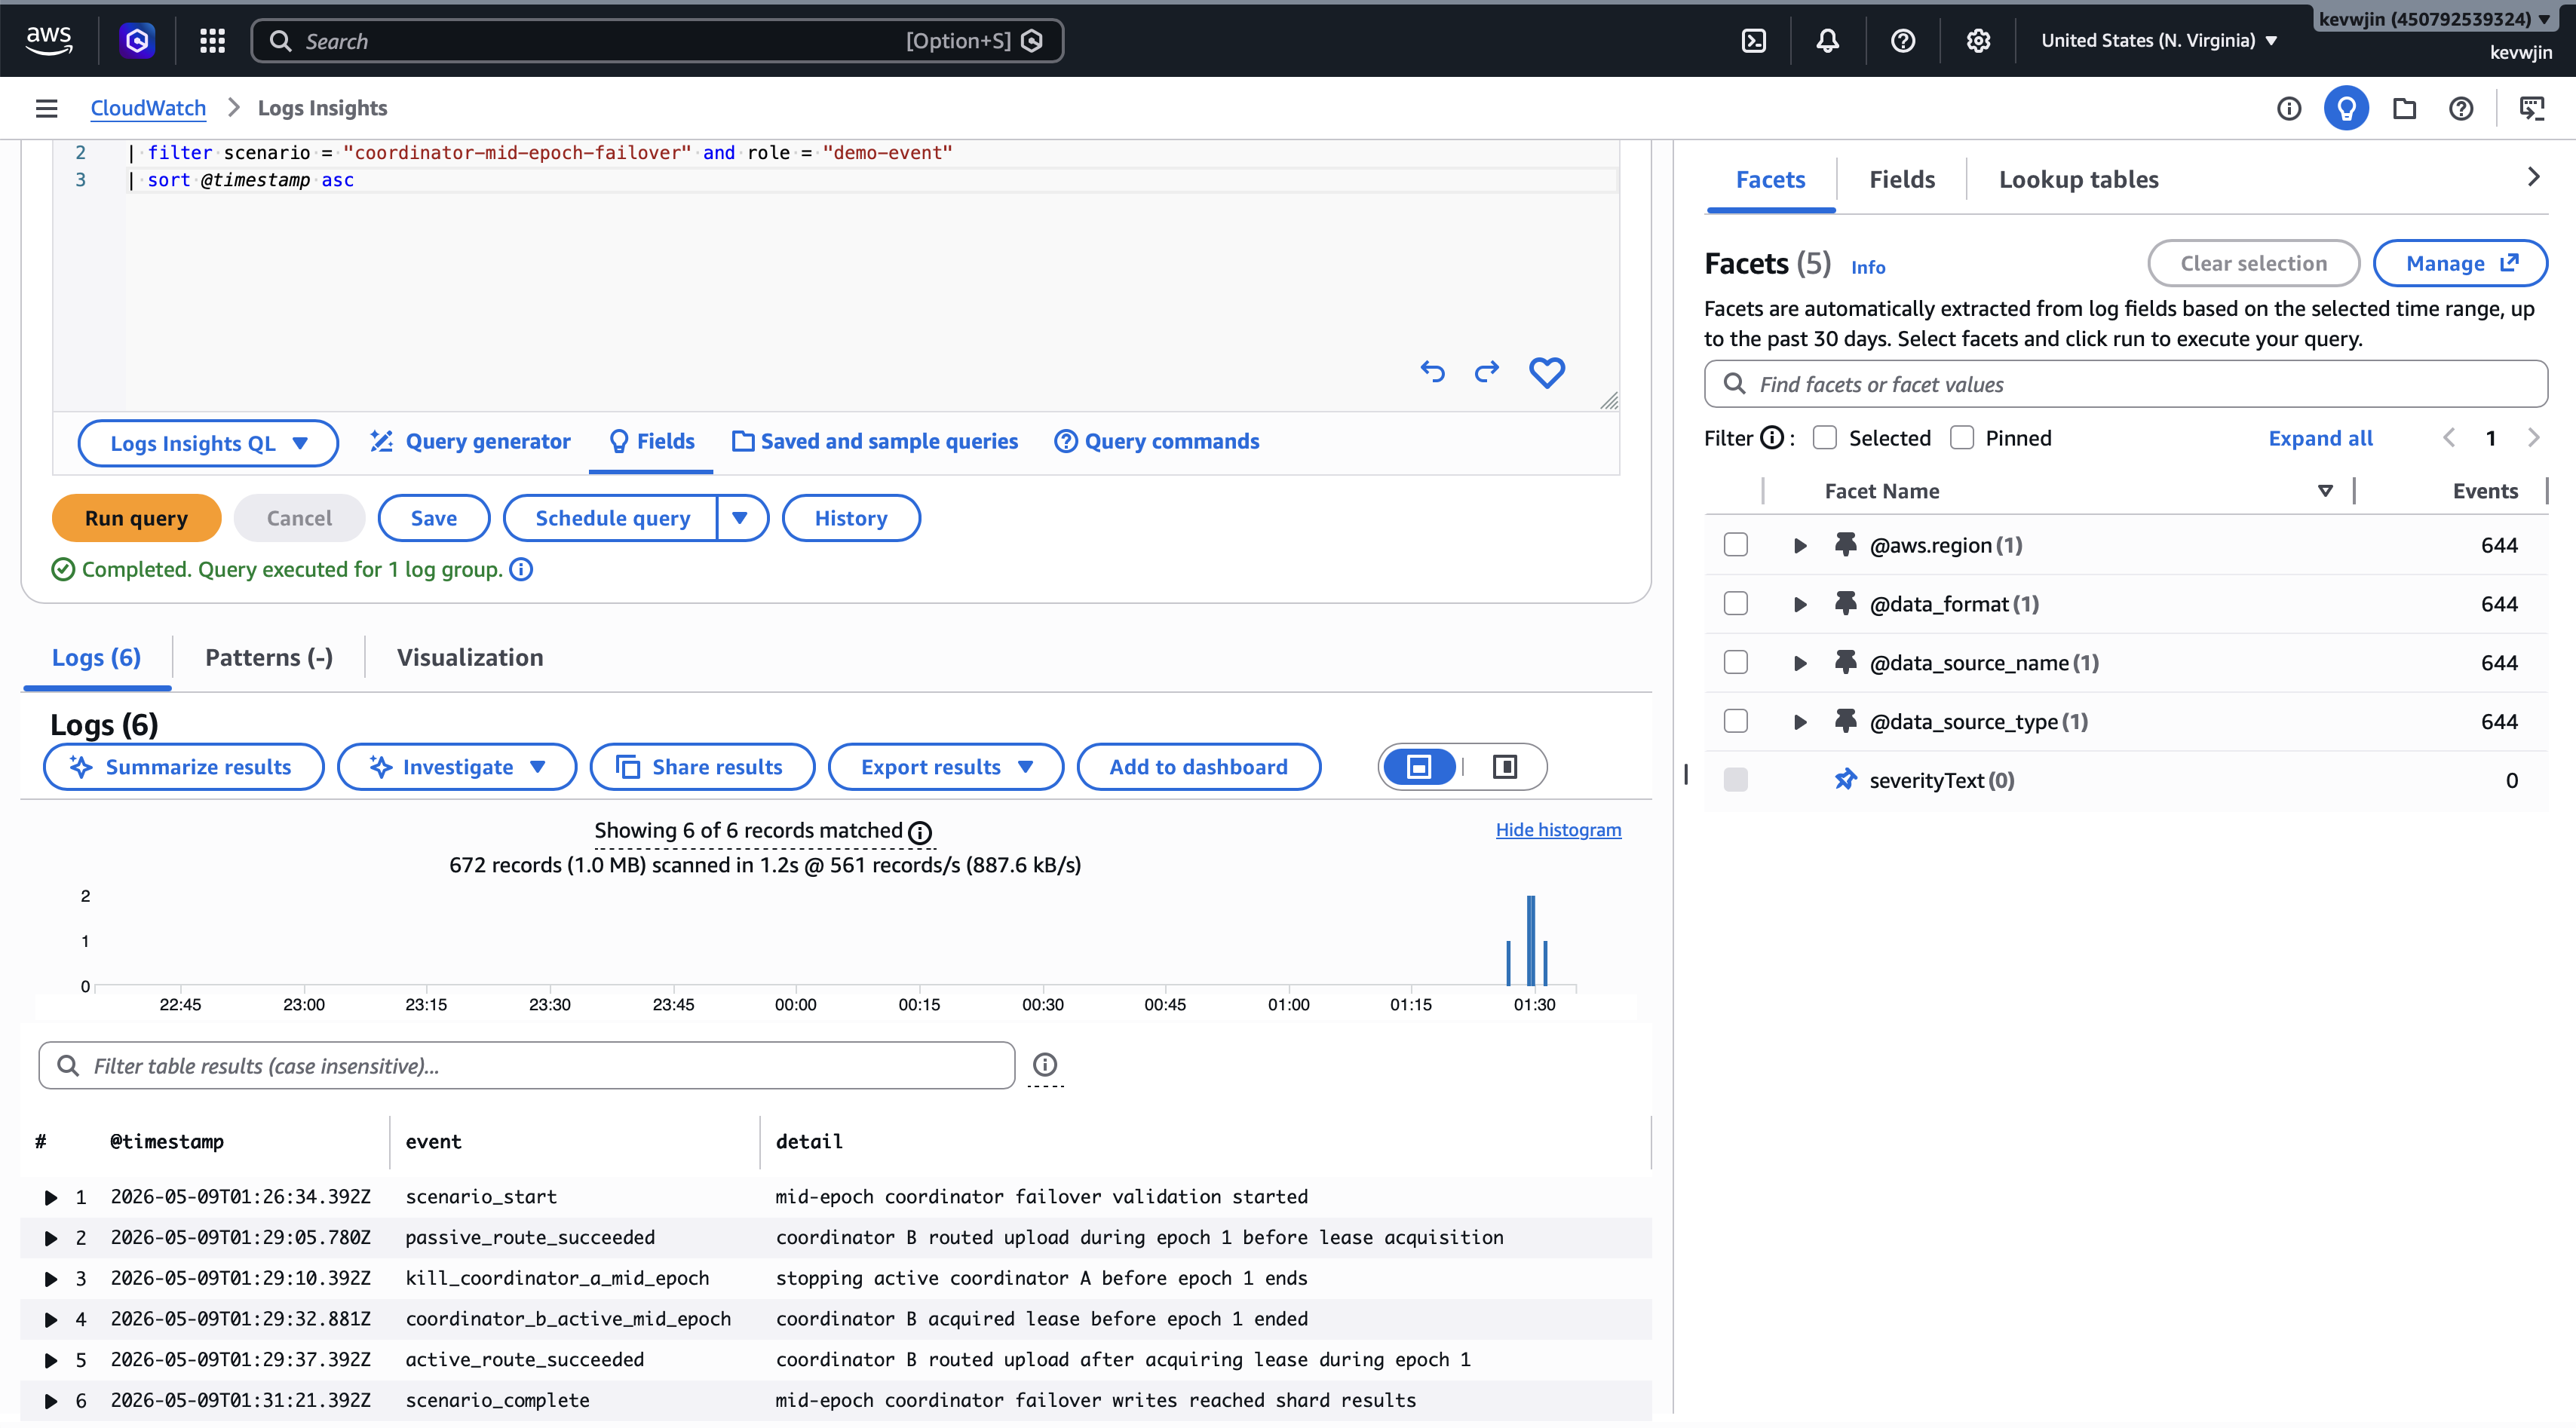
\includegraphics[width=\textwidth]{figures/failure-coordinator-events.png}
\caption{Coordinator failover event log. CloudWatch Logs Insights shows passive routing by coordinator B, termination of active coordinator A, B's mid-epoch lease acquisition, a post-acquisition routed write, and scenario completion.}
\label{fig:failure-coordinator-events}
\end{figure*}

Figure~\ref{fig:failure-coordinator-status} provides status-poller evidence for the same run. The visible columns include coordinator target, role, lease holder, lease active flag, and active holder. Early rows show coordinator A as \texttt{active} with a live lease and coordinator B as \texttt{passive}. After A stops renewing, subsequent status records show B taking over the active holder. The run output recorded distinct lease holder IDs for A and B, and the validation script completed with the message that AWS mid-epoch coordinator failover passed. The retained leader result files confirm that the routed writes reached shard results.

\begin{figure*}[!t]
\centering
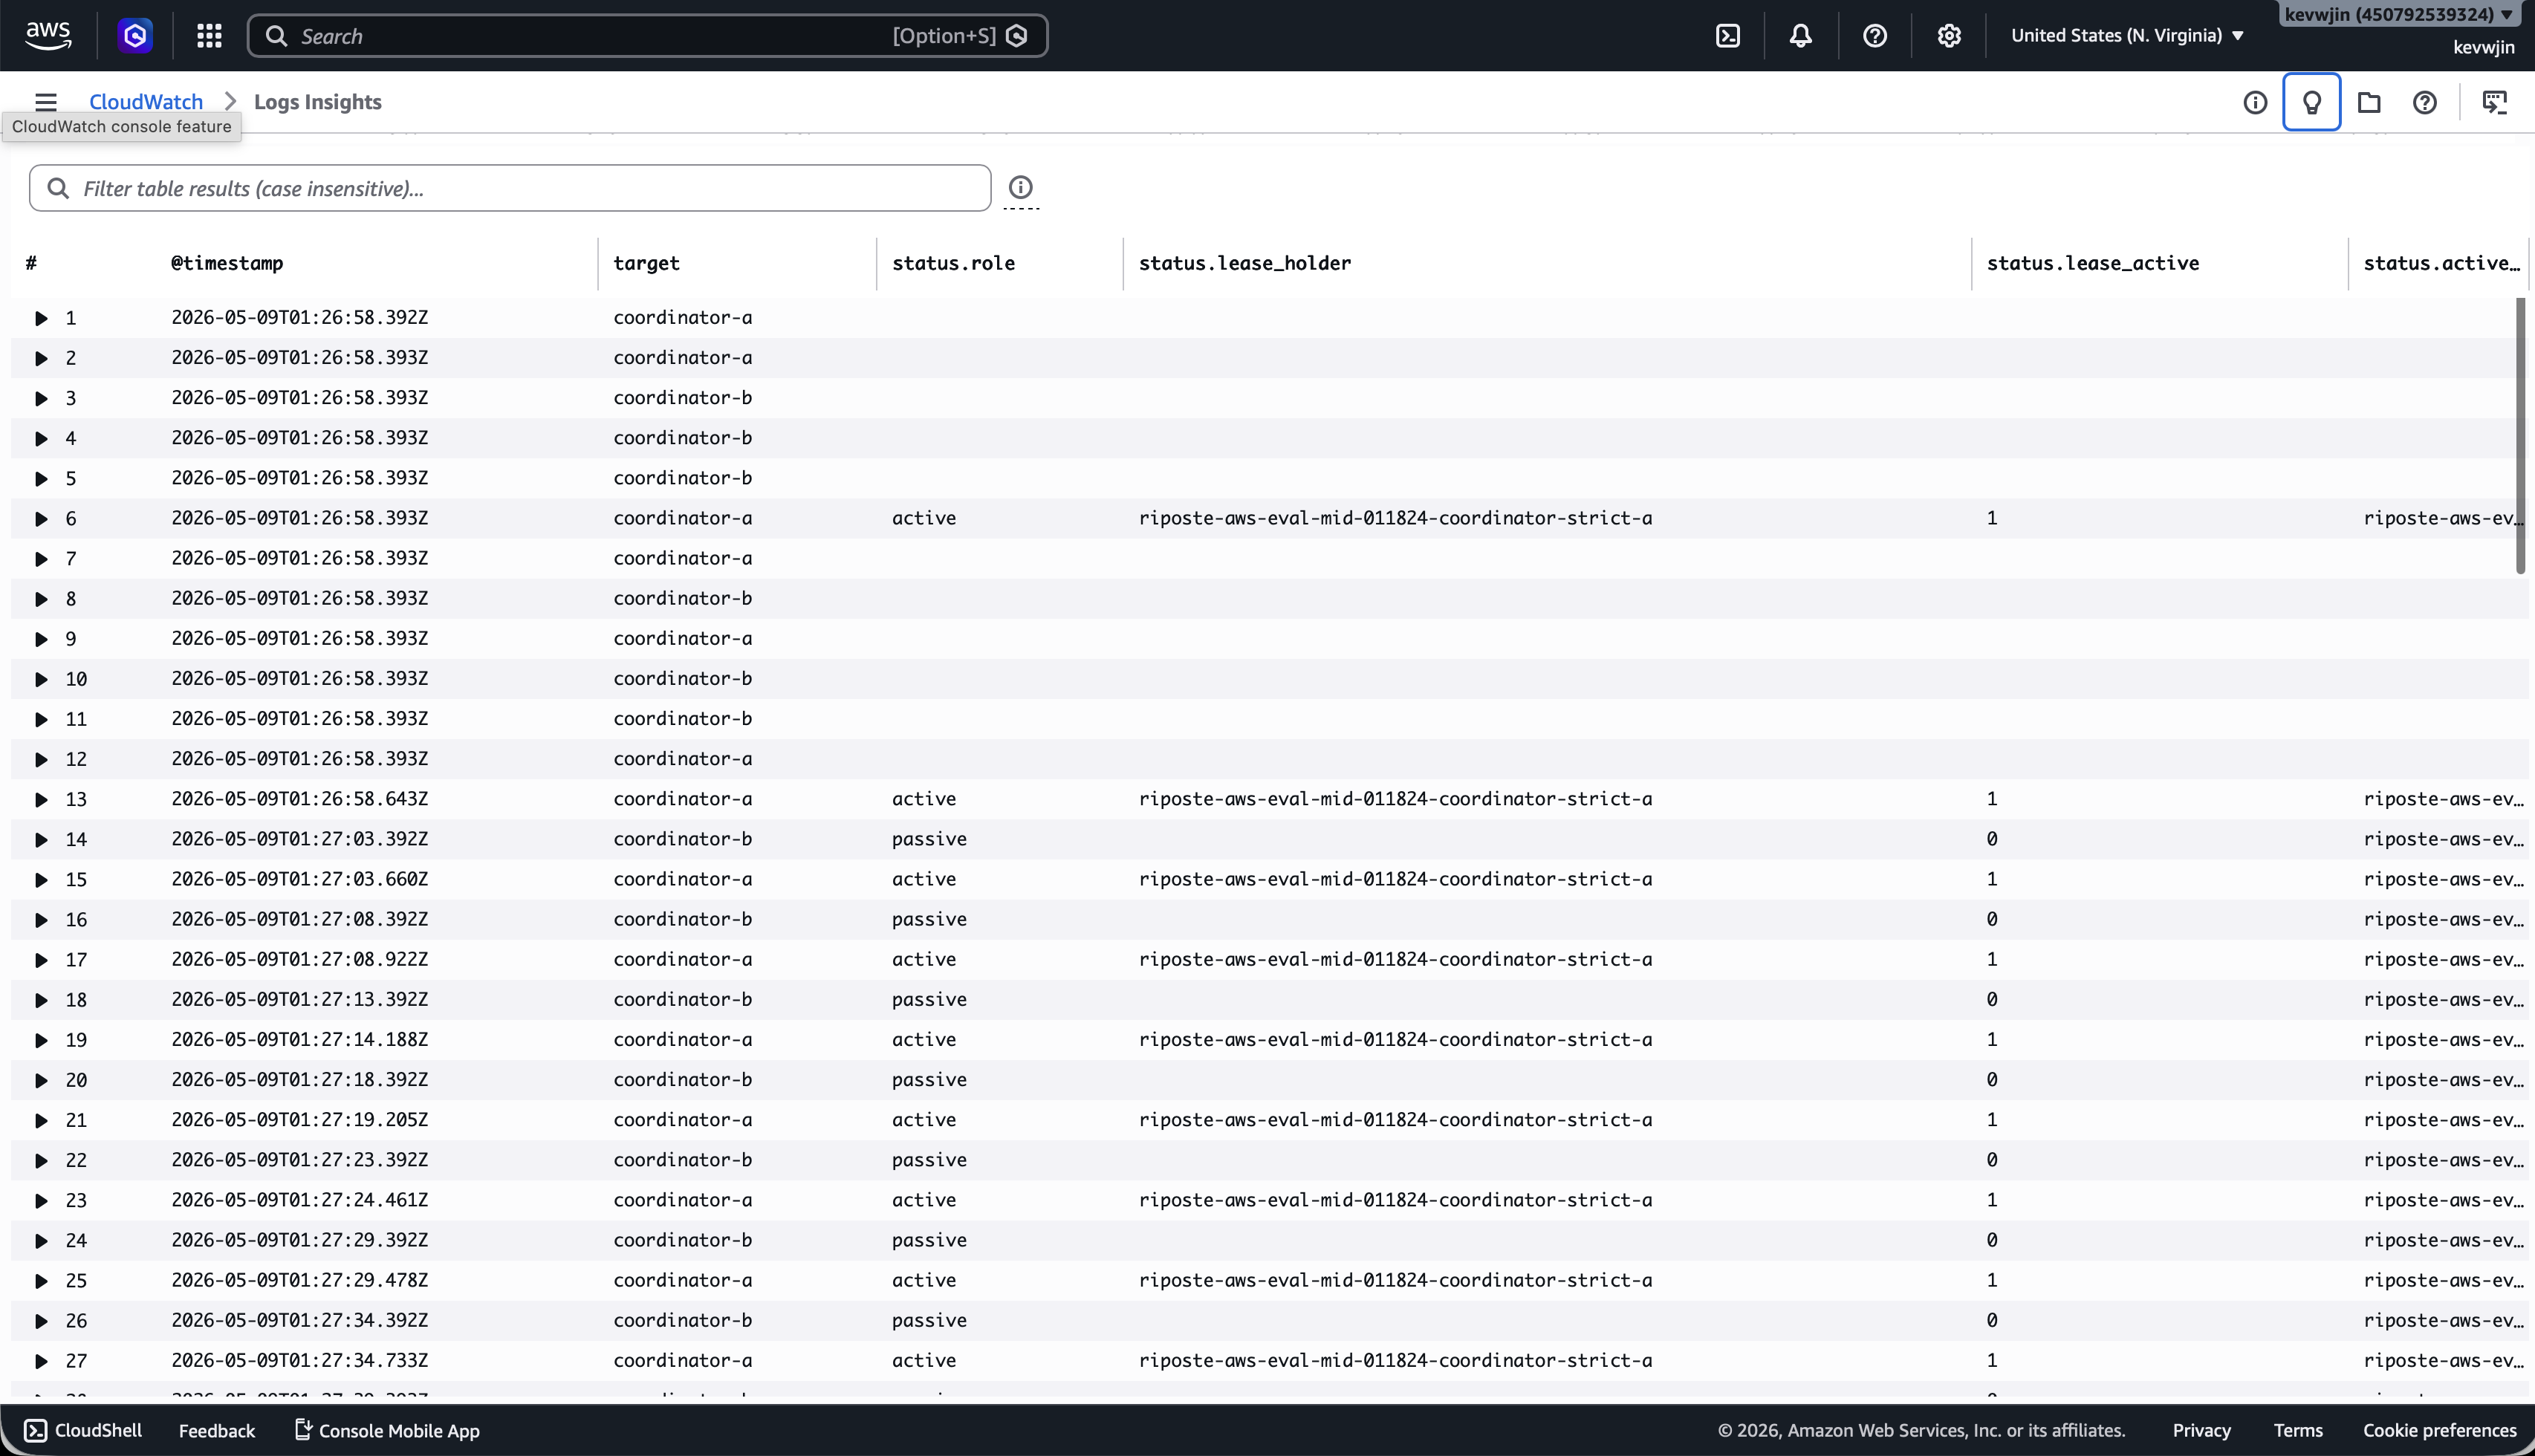
\includegraphics[width=\textwidth]{figures/failure-coordinator-status.png}
\caption{Coordinator lease and role status around failover. Status poller rows show coordinator A initially active with a live lease and coordinator B passive before the lease holder changes.}
\label{fig:failure-coordinator-status}
\end{figure*}

\paragraph{Recovery mechanism}
The recovery mechanism is the separation of data-plane routing from control-plane authority. DynamoDB stores the coordinator lease, lease expiry, and fencing token. While coordinator A is healthy, it renews the lease. Coordinator B stays alive and periodically attempts acquisition. When A is killed, renewal stops; after the lease expires, B acquires a newer fencing token and becomes authoritative. Upload routing can continue because upload sessions, epoch state, accepting state, and topology are shared through DynamoDB. Non-authoritative coordinators are blocked from lease-gated control mutations, but they may still route \texttt{Upload1}/\texttt{Upload2}/\texttt{Upload3} when the shared control store reports an active accepting epoch.

\paragraph{Limitations}
This scenario demonstrates coordinator failover, not shard failure recovery. The system still depends on DynamoDB for lease, epoch, topology, and session state. Control-plane operations can pause during the lease timeout before the standby becomes authoritative. Client RPCs that were in flight to the killed coordinator can fail and must be retried through the NLB/client retry path. The experiment validates the observed workload and timing, but it does not prove all high-concurrency races under arbitrary failure timing.

\subsection{Active Shard Leader Failure and Standby Promotion}

\paragraph{Failure definition}
The second scenario kills the active leader for shard 0. Before injection, active and standby shard replicas are both running. The system first warms the standby ingestion path during epoch 1, then stops the active shard 0 leader. The coordinator health loop detects that the active leader is unreachable, verifies that the standby is reachable and caught up, and updates the current shard topology so the standby leader becomes authoritative for shard 0. A later write to row 0 is expected to route to the promoted standby.

\paragraph{Observed behavior and evidence}
Figure~\ref{fig:failure-shard-promotion-events} shows the CloudWatch demo-event log for \texttt{scenario = "shard-auto-promotion"}. The sequence is \texttt{scenario\_start}, \texttt{kill\_shard0\_active}, \texttt{shard0\_auto\_promoted}, and \texttt{scenario\_complete}. The event details state that the active shard 0 leader was stopped, the control-store shard configuration switched to the standby leader, and a post-promotion write reached the promoted standby. The local validation artifacts recorded the pre-promotion epoch as 1 and the auto-promoted epoch as 2. The post-promotion shard configuration snapshot showed version 2 with shard 0's active leader address changed to the standby leader port, and the promoted shard result file confirmed that the post-promotion write was published.

\begin{figure*}[!t]
\centering
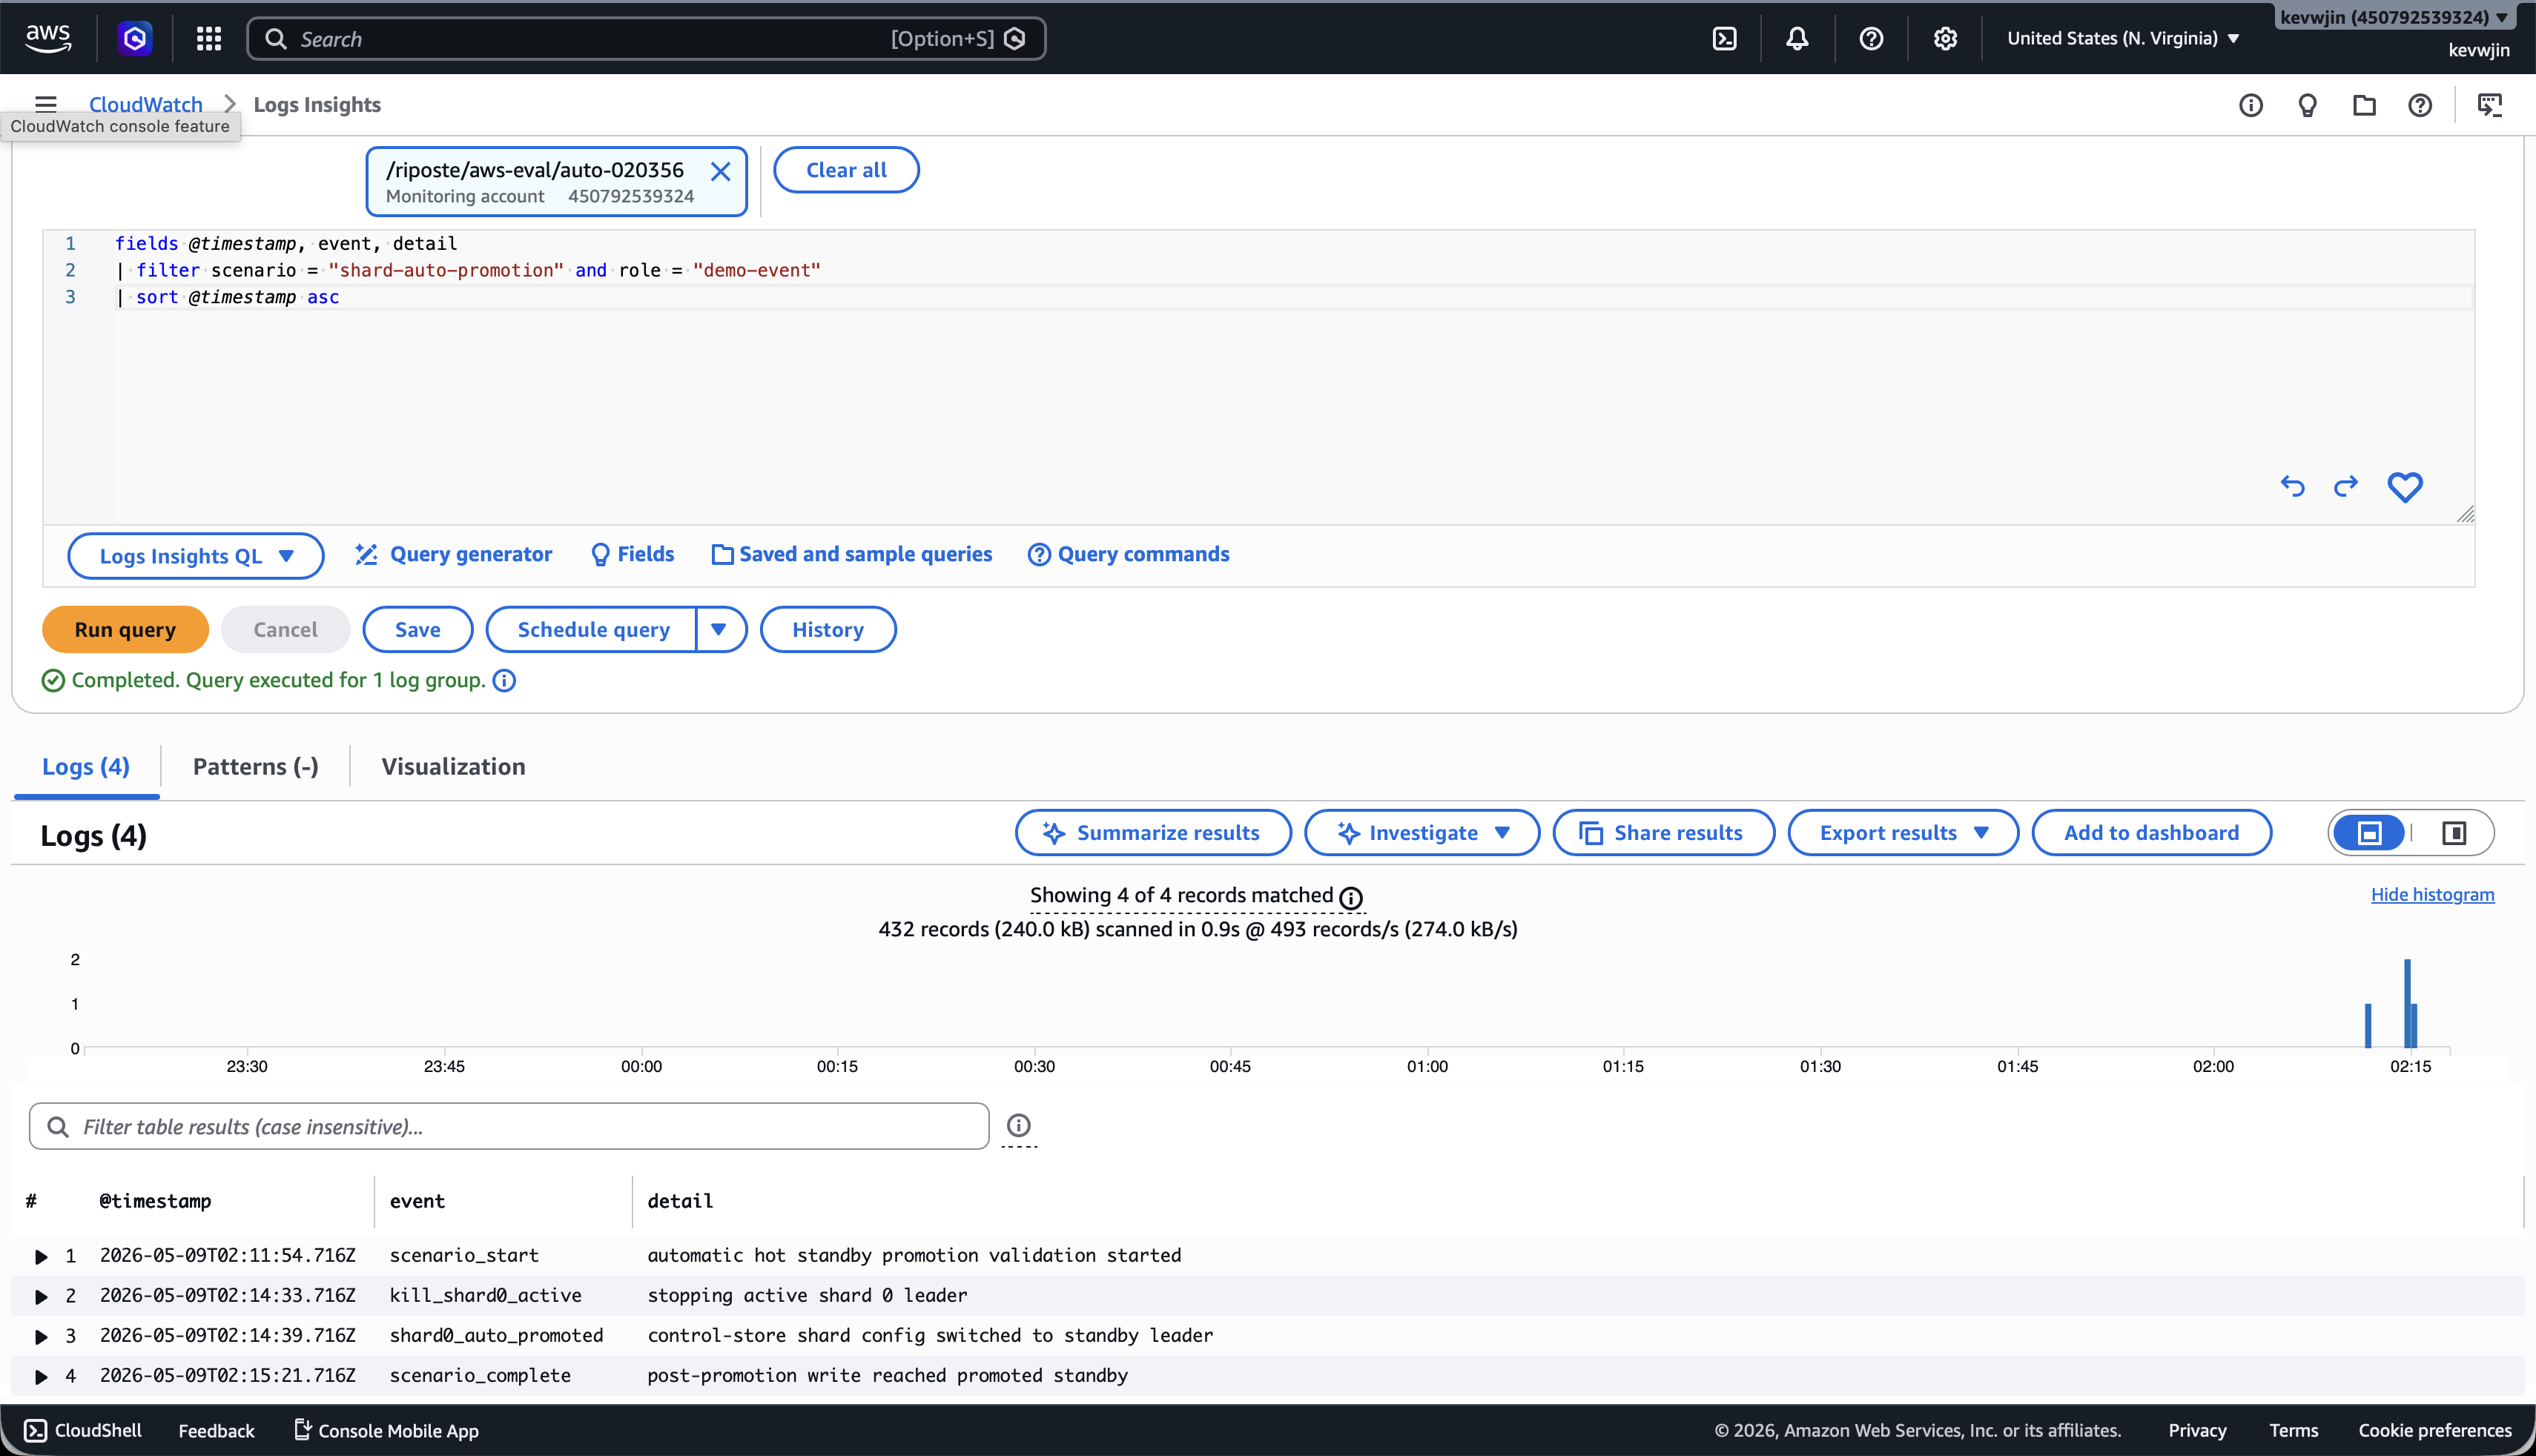
\includegraphics[width=\textwidth]{figures/failure-shard-promotion-events.png}
\caption{Automatic shard promotion event log. CloudWatch events show active shard 0 termination, automatic promotion of the standby leader in the control-store topology, and a successful post-promotion write.}
\label{fig:failure-shard-promotion-events}
\end{figure*}

\paragraph{Recovery mechanism}
Shard recovery uses hot standby ingestion and conservative topology mutation. After \texttt{Upload3} succeeds, the shard leader stores the completed-upload payload in S3 and sends pointer messages to the active and standby shard ingestion queues. The active and standby workers process the same completed-upload pointer independently and record replica-specific committed state in the completed-upload ledger. Because the standby is already consuming its own queue, it is hot rather than idle.

The coordinator health loop monitors active and standby reachability. Automatic promotion is guarded by a failure threshold and cooldown. The coordinator promotes only after the active shard fails consecutive checks and the standby is reachable, configured as a standby replica, queue-drained, error-free, and caught up according to ingestion and ledger counters. Promotion updates the current \texttt{shard-config} record in DynamoDB, swapping the standby address into the active slot and incrementing the topology version. Immutable epoch snapshots are not rewritten; future epochs and routes use the new current topology.

\paragraph{Limitations}
Promotion is not seamless for every possible in-flight upload. Partial shard-side \texttt{Upload1}/\texttt{Upload2} state can be lost when the active shard dies, because the durable replay boundary starts after accepted \texttt{Upload3}. Clients recover from that case by retrying the upload from \texttt{Upload1} after receiving the precise shard-session-loss signal. Hot standby also has ongoing cost because standby processes and queues run continuously. The readiness check uses live status counters and queue state; durable proof of standby progress across standby process restarts would require additional per-epoch replica progress records. The demonstrated failure model is active-unreachable failure, not Byzantine behavior or silent data corruption.

\subsection{Queue Ack Failure and Idempotent Redelivery}

\paragraph{Failure definition}
The third scenario models a common distributed-systems ambiguity: a worker processes a message successfully, but deleting the queue message fails. The server is started with the demo-only flag that forces one ingestion acknowledgement failure. A client write reaches \texttt{Upload3}; the shard stores the completed-upload payload in S3 and enqueues an SQS pointer. The worker loads the payload, processes the upload, and marks the completed-upload ledger committed. The first SQS ack/delete is then deliberately failed, so the message remains visible for redelivery after the visibility timeout.

\paragraph{Observed behavior and evidence}
Figure~\ref{fig:failure-sqs-events} shows the CloudWatch event log for the SQS idempotence scenario. The successful sequence includes \texttt{scenario\_start}, \texttt{upload\_start}, \texttt{queue\_drained}, and \texttt{scenario\_complete}. The screenshot also contains earlier retries from the same demonstration, so the important evidence is the final successful sequence in which the queue drained after redelivery. The event detail for \texttt{queue\_drained} states that SQS redelivery was acked after a ledger duplicate skip.

\begin{figure*}[!t]
\centering
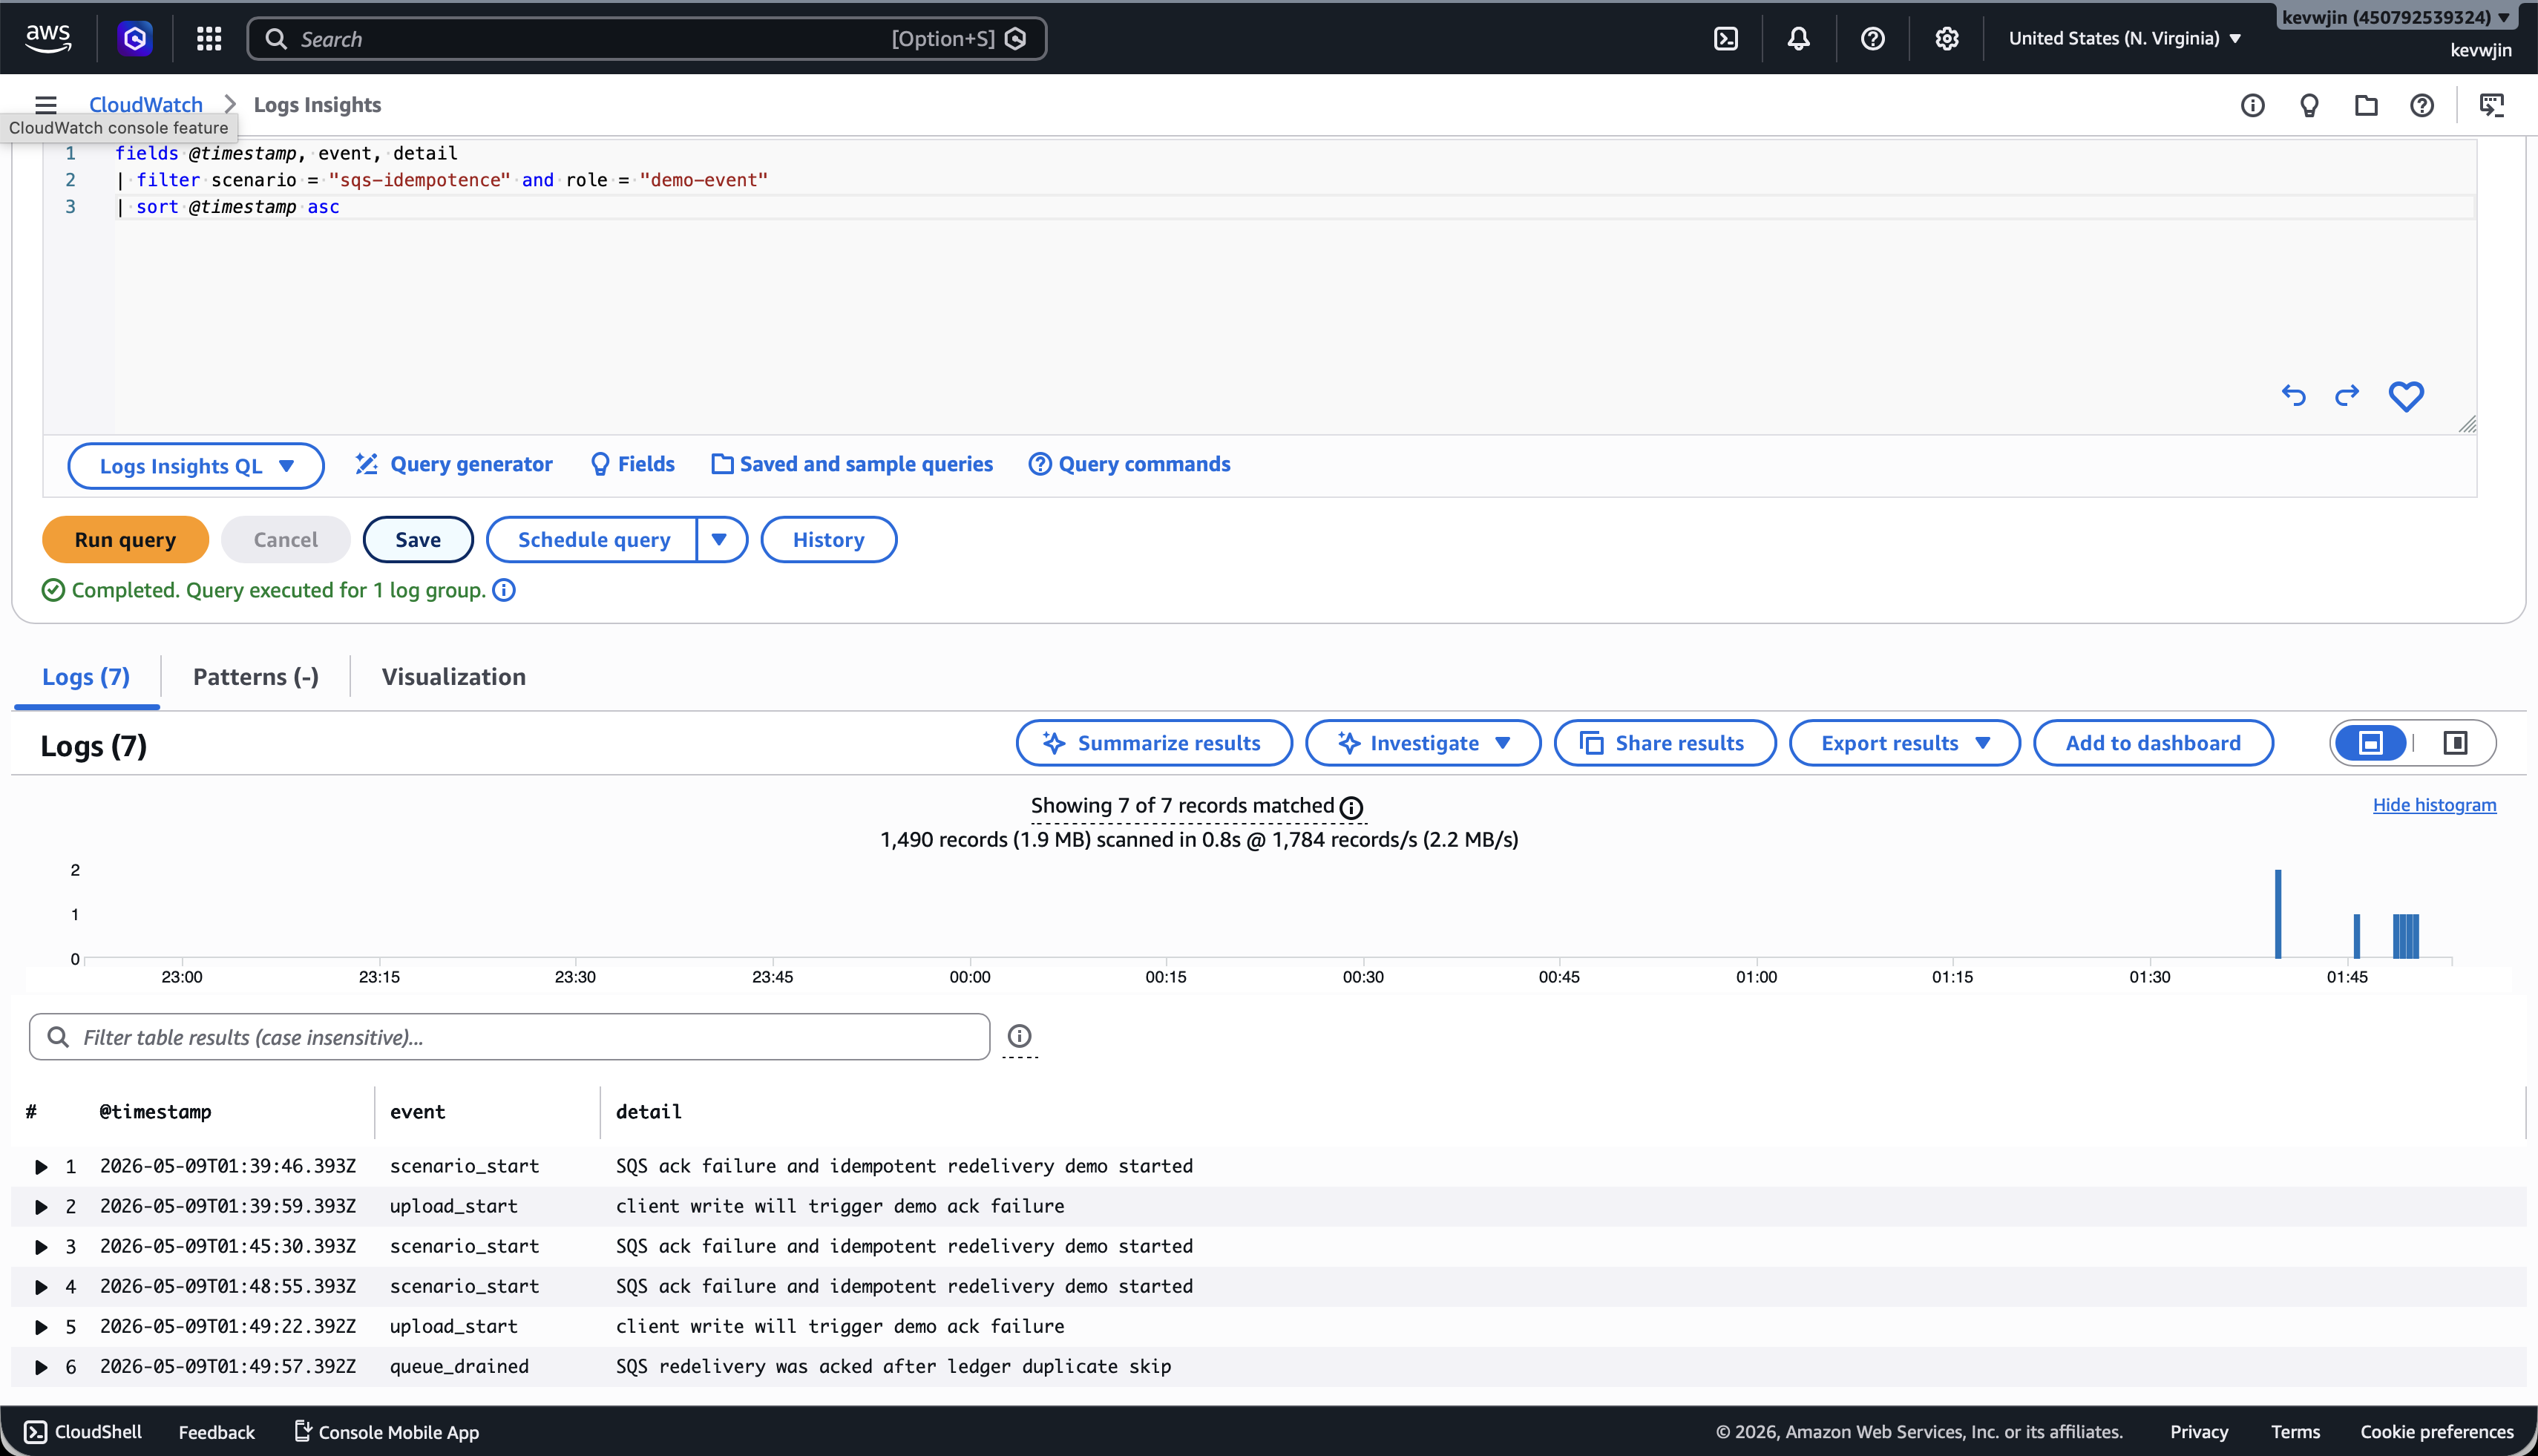
\includegraphics[width=\textwidth]{figures/failure-sqs-events.png}
\caption{SQS idempotence event log. CloudWatch events show the ack-failure demonstration, upload start, queue drain after redelivery, and scenario completion.}
\label{fig:failure-sqs-events}
\end{figure*}

Figure~\ref{fig:failure-sqs-counters} shows shard status counters for the same run. The key evidence is the \texttt{shard0-active} row: \texttt{ingestion\_ack\_error\_count = 1}, \texttt{completed\_upload\_duplicate\_skip\_count = 1}, \texttt{ingestion\_ack\_count = 1}, \texttt{ingestion\_queue\_depth = 0}, and \texttt{ingestion\_inflight\_count = 0}. These counters show that the injected ack failure occurred, the redelivered message was recognized as a duplicate using the ledger, the duplicate was eventually acknowledged, and no visible or in-flight queue work remained.

\begin{figure*}[!t]
\centering
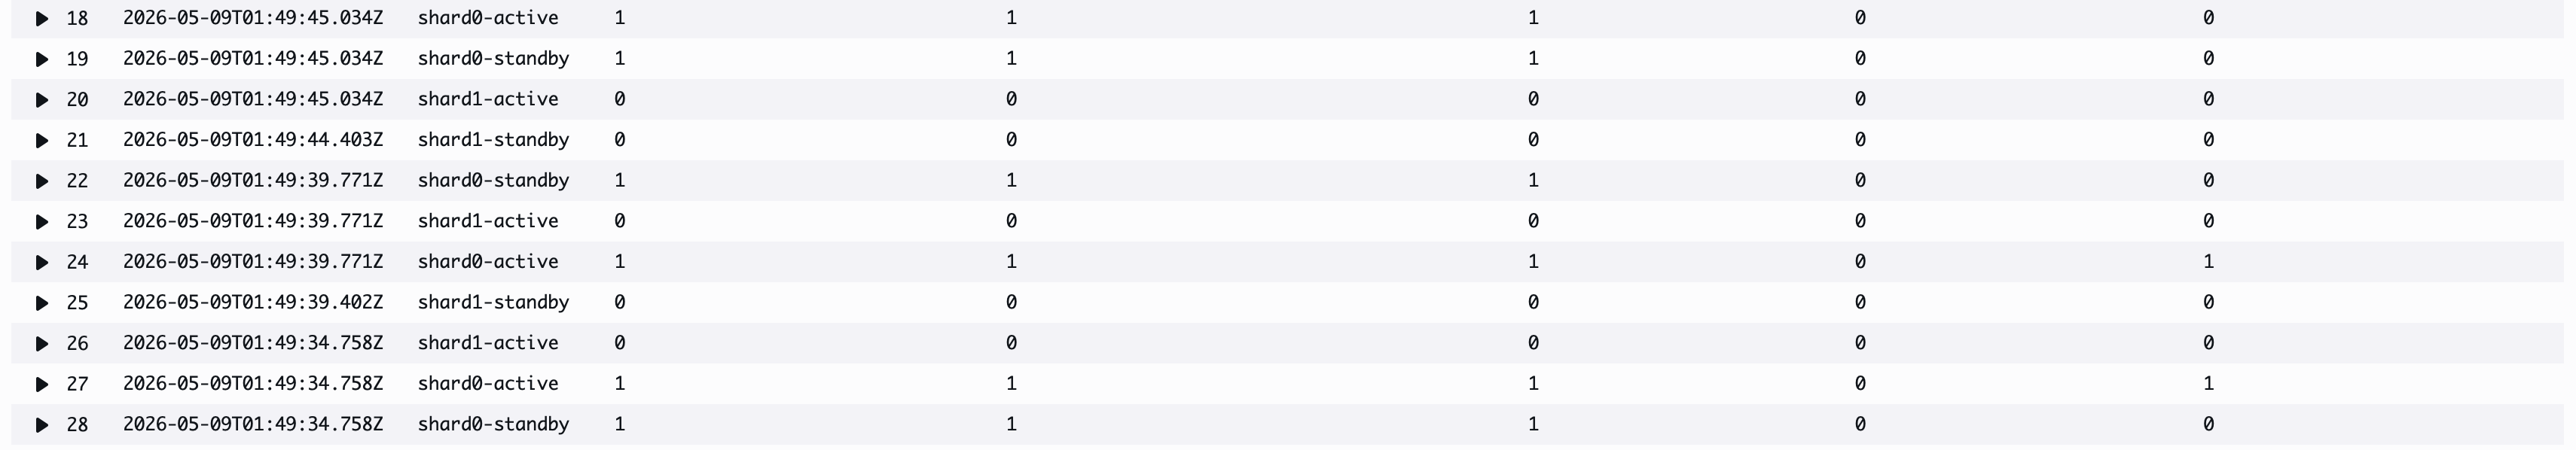
\includegraphics[width=\textwidth]{figures/failure-sqs-counters.png}
\caption{SQS idempotence counters. Shard status output shows one forced acknowledgement error, one duplicate skip, one eventual acknowledgement, and empty queue/in-flight counts.}
\label{fig:failure-sqs-counters}
\end{figure*}

\paragraph{Recovery mechanism}
The recovery mechanism combines S3 payload durability, SQS redelivery, and a completed-upload ledger. The SQS message carries a pointer to the S3 object rather than the full completed-upload payload. The worker reads the S3 object, performs prepare/commit processing, and records a ledger entry keyed by shard, epoch, upload UUID, and replica. Only after that does it attempt to ack/delete the SQS message. If deletion fails, SQS redelivers the pointer after the visibility timeout. On redelivery, the worker checks the ledger before repeating commit work. If the ledger already records the upload as committed for that replica, the worker skips duplicate processing and acknowledges the message.

\paragraph{Limitations}
This is pragmatic idempotence, not global exactly-once processing. It covers the important window where processing and ledger commit succeed before SQS acknowledgement fails. A crash after shard-local commit but before ledger commit remains a gap unless the shard commit itself becomes durably idempotent or is logged before mutation. S3 payload cleanup is also a separate policy decision. SQS ordering is not the main correctness property; duplicate detection through the ledger is. As in the shard-promotion scenario, partial \texttt{Upload1}/\texttt{Upload2} replay remains outside the durable completed-upload boundary.

\subsection{Cross-Scenario Discussion}

Across the three scenarios, the system deliberately uses different mechanisms for different failure domains. Coordinator failover is handled by DynamoDB lease/fencing and shared coordinator sessions. Shard failover is handled by hot standby ingestion, health checking, and topology promotion. Queue-processing ambiguity is handled by redelivery plus ledger-based duplicate detection. These are conservative mechanisms: they prefer explicit authority, durable state, and retryable work boundaries over attempting to hide every failure from the client.

The most important boundary is \texttt{Upload3}. After accepted \texttt{Upload3}, the system has a durable completed-upload payload, SQS pointer messages, and ledger-backed processing. Before that point, the protocol still contains interactive client/shard state. This is why coordinator failover can preserve upload routing through shared sessions, while shard promotion may still require clients to restart a partially completed upload if the active shard dies before the durable ingestion boundary.

The remaining limitations point to future work. The system would benefit from durable partial-session replay for \texttt{Upload1}/\texttt{Upload2}, stronger idempotence around local shard commit plus ledger commit, durable per-epoch standby progress records, automated replacement of standby capacity after promotion, and broader high-concurrency failure testing. These limitations do not invalidate the demonstrated recovery behavior, but they constrain the claims: the evaluation proves bounded coordinator failover, hot-standby shard promotion, and safe redelivery after an ack failure, not arbitrary exactly-once or Byzantine-fault-tolerant operation.

\section{Performance \& Scalability Evaluation}

\subsection{Workload Methodology}

The performance evaluation follows the same interpretation used in the Riposte reproduction paper: it measures accepted upload throughput under hammer load, not realistic message recoverability. Hammer mode is a stress workload. Each worker repeatedly submits uploads to keep the online write-validation path busy, so the benchmark is useful for comparing processing capacity but should not be interpreted as evidence that every accepted upload would become a uniquely recoverable message in a realistic epoch.

The primary comparison used one AWS run in \texttt{us-east-1} on the same c7i deployment family. The baseline phase sent clients directly to a single leader/follower shard pair. The sharded phase sent clients through the coordinator, which routed uploads across two active shard pairs. Both phases used a 60-second warm-up epoch followed by a 600-second measured epoch. The measured configuration used two server threads per shard server, one client thread, client concurrency 16, and overload retry enabled with 10 ms initial and 250 ms maximum backoff. The primary metric is accepted uploads per second, derived from server-side accepted-count logs.

\subsection{Write Throughput}

Table~\ref{tab:write-throughput} summarizes the same-run comparison. The direct single-shard baseline accepted 38,908 uploads, or 64.85 requests/s. The sharded coordinator path accepted 79,024 uploads, or 131.71 requests/s. This is an increase of 40,116 accepted uploads, or 103.10\%. The result should be read as near-linear two-shard scaling. The small amount above exactly \(2\times\) is best explained by measurement-window effects, backoff behavior, active-until estimates, and normal run-to-run variation rather than by a meaningful superlinear effect.

\begin{table}[!t]
\centering
\caption{Write throughput over a 600-second measured epoch}
\label{tab:write-throughput}
\small
\begin{tabular}{l r r}
\hline
\textbf{Deployment} & \textbf{Accepted uploads} & \textbf{Req/s} \\
\hline
Baseline & 38,908 & 64.85 \\
Sharded & 79,024 & 131.71 \\
\hline
\end{tabular}
\end{table}

The shard-level split explains the gain. Shard 0 accepted 39,518 uploads and shard 1 accepted 39,506 uploads. Each shard therefore processed approximately the same amount of work as the direct single-shard baseline. This supports the main scalability claim: row-range routing lets two independent shard pairs process the online Riposte validation path in parallel.

\subsection{Concurrency Sweep and Backpressure}

Before the long run, a short concurrency sweep was used to choose the load point. Table~\ref{tab:concurrency-sweep} reports accepted uploads and overload retries for the direct baseline and the sharded coordinator path. The sharded deployment improved accepted uploads at every tested concurrency. At higher concurrency, both configurations began to experience queue-full backpressure, but the baseline saw more overload retries because all pressure targeted one shard queue.

\begin{table*}[!t]
\centering
\caption{Short AWS client-concurrency sweep}
\label{tab:concurrency-sweep}
\small
\begin{tabular}{r r r r r}
\hline
\textbf{Concurrency} & \textbf{Baseline accepted} & \textbf{Sharded accepted} & \textbf{Delta} & \textbf{Overload retries base/shard} \\
\hline
1 & 2,816 & 4,121 & +46.34\% & 0 / 0 \\
2 & 2,877 & 4,662 & +62.04\% & 0 / 0 \\
4 & 2,884 & 5,205 & +80.48\% & 0 / 0 \\
8 & 3,423 & 5,747 & +67.89\% & 1,363 / 0 \\
16 & 3,238 & 6,261 & +93.36\% & 2,862 / 1,866 \\
\hline
\end{tabular}
\end{table*}

The server can return \texttt{server overloaded: ready queue full} when \texttt{Upload3} tries to enqueue a completed upload and the ready queue is full. In the benchmark, this is a backpressure signal rather than a server crash. The hammer client therefore used opt-in overload retry: it retried the same plaintext with exponential backoff, and the run was considered valid only if the client eventually exited through the expected \texttt{No active epoch} path. This methodology matches the reproduction paper's emphasis on accepted server-side throughput rather than client-perceived latency.

\subsection{Latency, Scaling Response, and Resource Limits}

The current Riposte write-path benchmark does not report P95 or P99 upload latency samples. This is consistent with the reproduction paper's performance framing, which focuses on accepted upload throughput, throughput stability, and backpressure behavior. The system is epoch-based and latency-tolerant, so the more relevant user-visible delay is the epoch duration plus publication time rather than per-RPC response latency. Future work should add per-upload latency instrumentation if the goal is to compare client-perceived responsiveness across coordinator, NLB, and shard configurations.

The scaling response measured here is architectural rather than automatic EC2 provisioning latency. Completed epochs produce accepted-request-density recommendations, and a recommendation can be applied only between epochs. This preserves stable shard anonymity sets and avoids changing row routing while an epoch is accepting writes. The evaluated throughput result therefore demonstrates the benefit once two shard pairs are active; it does not yet measure the time to launch new EC2 shard capacity.

The bottleneck is the online write-validation and admission path. Sharding improves throughput because it splits the ready-queue pressure and validation work across independent shard pairs. The benchmark does not include complete per-instance CPU, memory, disk, or network graphs, so resource utilization must be interpreted conservatively. Queue-full retries show that admission pressure exists under high offered load, and the fact that both shards process near-baseline work suggests that additional shards should improve throughput approximately linearly until another bottleneck, such as client generation, coordinator routing, DynamoDB session traffic, or network capacity, becomes dominant.

\section{Cost Analysis}

\subsection{Deployment Cost Estimate}

The cost model has two parts: a fixed deployment cost dominated by compute and ingress, and a variable cost driven primarily by completed-write volume. The AWS demo deployment used one coordinator EC2 instance, one client/load-generator instance, and four shard EC2 instances for two leader/follower shard pairs. It also used one Network Load Balancer, one DynamoDB table for control, session, topology, recommendation, and ledger records, one S3 bucket for completed-upload payloads and published artifacts, and SQS queues for shard ingestion. With hot standby ingestion enabled, each shard uses two queues: one active queue and one standby queue. A two-shard deployment therefore has four SQS queues.

The functional AWS demonstrations used \texttt{t3.small} instances to avoid quota issues. AWS lists T3 Linux prices for US East (N. Virginia) on the T3 instance page, with \texttt{t3.small} currently approximately \$0.0209 per hour in that region~\cite{awst3}. For six instances, the EC2 compute component is therefore \(6 \times \$0.0209 \approx \$0.1254\) per hour. Using a 730-hour month, this is approximately \(\$0.1254 \times 730 \approx \$91.54\) per month if the demo stack is left running continuously. This estimate excludes EBS, data transfer, taxes, and free-tier credits. It also changes with region, operating system, instance family, purchase option, and whether the deployment uses benchmark instances such as \texttt{c7i.large}.

The NLB adds a second fixed cost component. AWS bills Network Load Balancers by load balancer hours and Network Load Balancer Capacity Units (NLCUs)~\cite{awselb}. For this prototype, the NLB cost is mostly a fixed hourly charge at small scale because the measured traffic is modest compared with the NLCU dimensions. DynamoDB, SQS, S3, and CloudWatch are request- or storage-driven in the demo. Their costs are small for short validation runs, but they become important in a sustained write-heavy deployment.

\subsection{Scaling Cost Behavior}

Shard scaling grows cost approximately linearly with the number of active shards. Let \(S\) be the number of active shards and let \(R\) be the replica factor used for ingestion. In an active-only configuration, \(R=1\). With hot standby ingestion, \(R=2\) because both the active and standby replicas consume completed-upload pointers. If every active shard pair runs on separate EC2 hosts, then the shard compute component is roughly proportional to \(2S\) EC2 instances for leader/follower pairs. If hot standby replicas are deployed as additional processes on the same hosts, the hourly instance count does not immediately double, but CPU headroom, memory pressure, and queue-processing work still increase.

The queue count is \(Q_{\mathrm{SQS}} = R \times S\). For the demonstrated two-shard hot-standby deployment, \(Q_{\mathrm{SQS}} = 2 \times 2 = 4\) queues. More importantly, completed-upload request volume also multiplies by \(R\). For \(W\) completed uploads, the ingestion path writes \(W\) S3 payload objects. It then sends \(R W\) SQS pointer messages, performs approximately \(R W\) SQS receives and \(R W\) SQS deletes in the no-redelivery case, and performs \(R W\) S3 reads as workers load the payloads. Ignoring long-poll empty receives and redeliveries, the SQS request count is approximately \(N_{\mathrm{SQS}} \approx 3 R W\). Active-only ingestion is about \(3W\) SQS API requests, while hot standby ingestion is about \(6W\). Redelivery, polling when queues are empty, and status checks add more requests.

DynamoDB request volume is also write-path dominated. Each upload creates and later deletes or updates coordinator session state, and each completed-upload replica writes or checks a completed-upload ledger record. For \(W\) completed uploads and replica factor \(R\), the ledger component alone is \(O(RW)\) DynamoDB write/check activity. Coordinator leases, epoch records, shard-config records, and scaling recommendations are low-rate control-plane traffic by comparison. This is why the cost profile is mostly on the write side: the system does expensive validation, durable enqueue, payload storage, replica processing, and ledger updates when admitting writes. Read serving primarily fetches already-published artifacts and does not run the interactive upload validation path.

CloudWatch cost scales with log volume and query volume. AWS bills CloudWatch Logs for ingestion, storage, and Logs Insights query scans~\cite{awscloudwatch}. The demo intentionally emits detailed status and event records for evidence, so debug-heavy validation can make CloudWatch a visible cost even when SQS, DynamoDB, and S3 usage remains small.

\subsection{Architectural Cost Trade-offs}

Hot standby is the main availability-versus-cost trade-off. It costs more than cold replay because standby processes run during normal operation and standby SQS queues receive the same completed-upload pointers as active queues. The benefit is faster promotion: the standby has already processed the completed-upload stream and can be promoted after health and catch-up checks. A cold replay design would reduce idle compute and queue activity, but recovery would require scanning S3 payloads, SQS state, or ledger history before promotion, increasing recovery time and operational complexity.

The S3-plus-SQS ingestion design is also a deliberate cost trade-off. Sending the full completed-upload payload through SQS would be simpler, but SQS charges by request and message payload chunks, and large payloads are constrained by queue message size. AWS SQS pricing is request based, and AWS notes that larger payloads are billed in 64 KB chunks~\cite{awssqs}. Storing the full payload in S3 and sending only an SQS pointer adds S3 PUT/GET/storage costs, but it keeps queue messages small, preserves durable audit artifacts, and makes replay independent of SQS message body size. AWS S3 pricing separately charges for storage and requests such as PUT and GET~\cite{awss3}.

DynamoDB trades per-request cost for operational simplicity. The prototype needs conditional point writes for leases, fencing tokens, shard topology, session records, and completed-upload ledgers. DynamoDB on-demand capacity bills by read and write request units and avoids operating a separate replicated metadata store~\cite{awsdynamodb}. A self-managed consensus system could reduce some managed-service request charges at high sustained volume, but it would add EC2 cost, operational complexity, monitoring burden, and its own failure modes.

The load balancers are fixed-cost ingress choices. The NLB adds hourly and capacity-unit charges, but it provides stable custom TCP ingress and lets clients reach multiple coordinator processes without embedding coordinator membership in the client. The ALB adds a separate ingress cost for stateless HTTP reads, but it reduces custom health-check and measurement code. CloudWatch is similarly valuable for demos and operations but should be configured with retention, sampling, and query discipline in production. The overall cost pattern is therefore clear: fixed cost comes from always-on EC2 and load-balancer resources, while variable cost grows with completed writes through S3 payloads, SQS pointer fanout, DynamoDB session/ledger operations, and CloudWatch logs.

\section{Testing}

The final AWS validation used structured tests covering the required functional, scaling, failure, security, and performance dimensions. These tests are intentionally different from the longer performance and failure-analysis sections: this section records whether each required behavior was exercised end-to-end in AWS and identifies the evidence artifact used to support the result. Table~\ref{tab:structured-tests} summarizes the test suite.

\begin{table*}[!t]
\centering
\caption{Structured AWS-backed test cases}
\label{tab:structured-tests}
\small
\begin{tabular}{p{0.08\textwidth} p{0.14\textwidth} p{0.31\textwidth} p{0.36\textwidth}}
\hline
\textbf{Test} & \textbf{Category} & \textbf{Purpose} & \textbf{Observed result} \\
\hline
T1 & Functional & Verify that a sharded epoch completes with deterministic writes and matched active/standby ingestion state. & Epoch 1 completed with global table height 512, two accepted deterministic writes, and active/standby committed counts of 1 and 1. \\
T2 & Scaling & Verify that accepted-request density can trigger and apply a grow recommendation between epochs. & A validation threshold made density 0.00390625 produce \texttt{grow}; shard count changed from 1 to 2, global height changed from 256 to 512, and the cycle reached \texttt{scaling\_applied}. \\
T3 & Failure & Verify shard hot-standby promotion and post-promotion write admission. & After the active shard 0 leader was stopped, the standby was promoted and a subsequent write reached the promoted standby. \\
T4 & Security & Verify AWS network isolation for evaluator access and internal application traffic. & SSH was restricted to the evaluator IP, and application traffic was scoped to the evaluation security group rather than opened broadly to the Internet. \\
T5 & Performance & Verify that sharding improves accepted upload throughput under the reproduction-style hammer benchmark. & The same-run AWS comparison accepted 38,908 baseline uploads and 79,024 sharded uploads, a 103.10\% increase. \\
\hline
\end{tabular}
\end{table*}

\subsection{T1 Functional: Completed Sharded Epoch}

The functional test checked the basic correctness path for the deployed sharded system. The workload wrote deterministic boundary-row messages through the coordinator, allowed the epoch to complete, and inspected CloudWatch evidence for the completed epoch state. Figure~\ref{fig:test-functional} shows that epoch 1 completed with a global table height of 512, meaning two 256-row shards were active. It also shows two accepted deterministic writes and matched active/standby committed counts. This verifies that the sharded write path, global-row routing, durable ingestion, and standby catch-up path were all exercised in the same AWS run.

\begin{figure*}[!t]
\centering
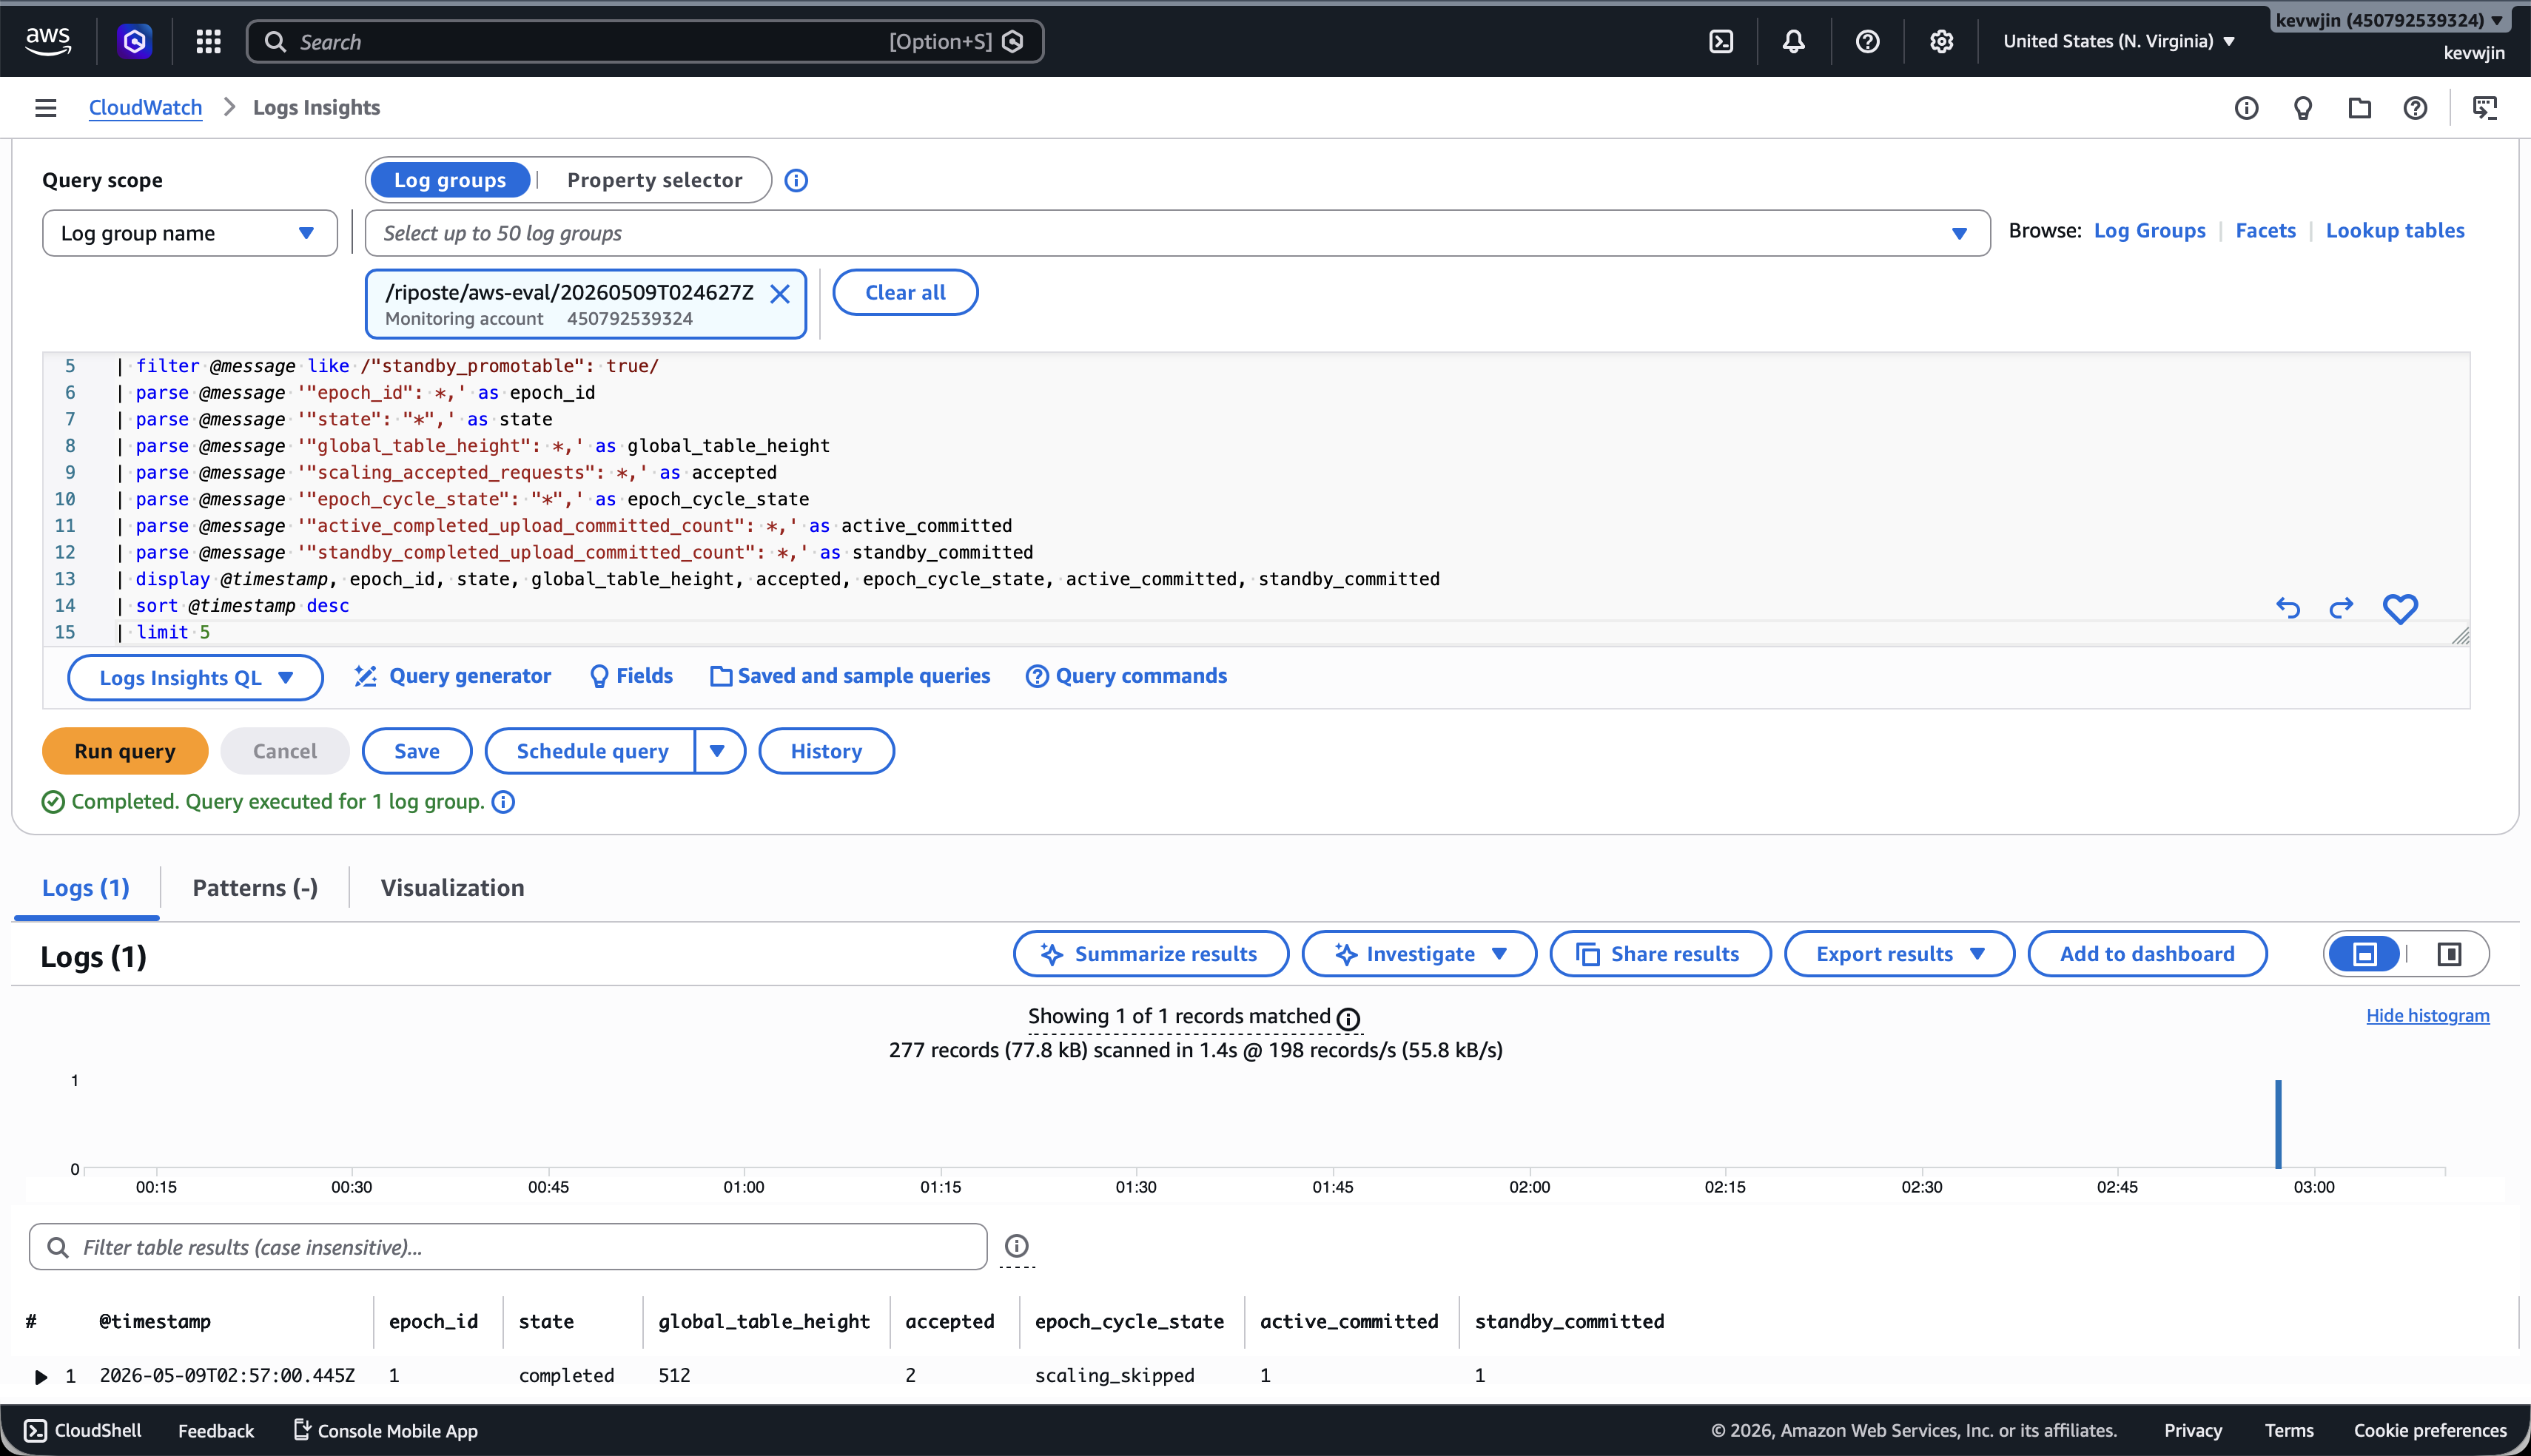
\includegraphics[width=0.95\textwidth]{figures/test-functional-completed-epoch.png}
\caption{T1 functional evidence: completed sharded epoch with two accepted deterministic writes and matching active/standby committed counts.}
\label{fig:test-functional}
\end{figure*}

\subsection{T2 Scaling: Grow Recommendation Applied}

The scaling test validated the density-to-apply path without requiring live EC2 provisioning. The run intentionally used an easier validation threshold so a short AWS test could trigger a grow recommendation without needing a long or expensive load run. The completed-epoch accepted-request density was 0.00390625, which produced action \texttt{grow} and recommended two shards. Applying that recommendation changed the authoritative shard configuration from one active shard to two active shards, increased global table height from 256 to 512, and moved the epoch cycle to \texttt{scaling\_applied}. Figure~\ref{fig:test-scaling} shows both the density evidence and the applied scaling state. This demonstrates that scaling recommendations are persisted separately, checked for applicability, and promoted into the next shard topology only at an epoch boundary.

\begin{figure*}[!t]
\centering
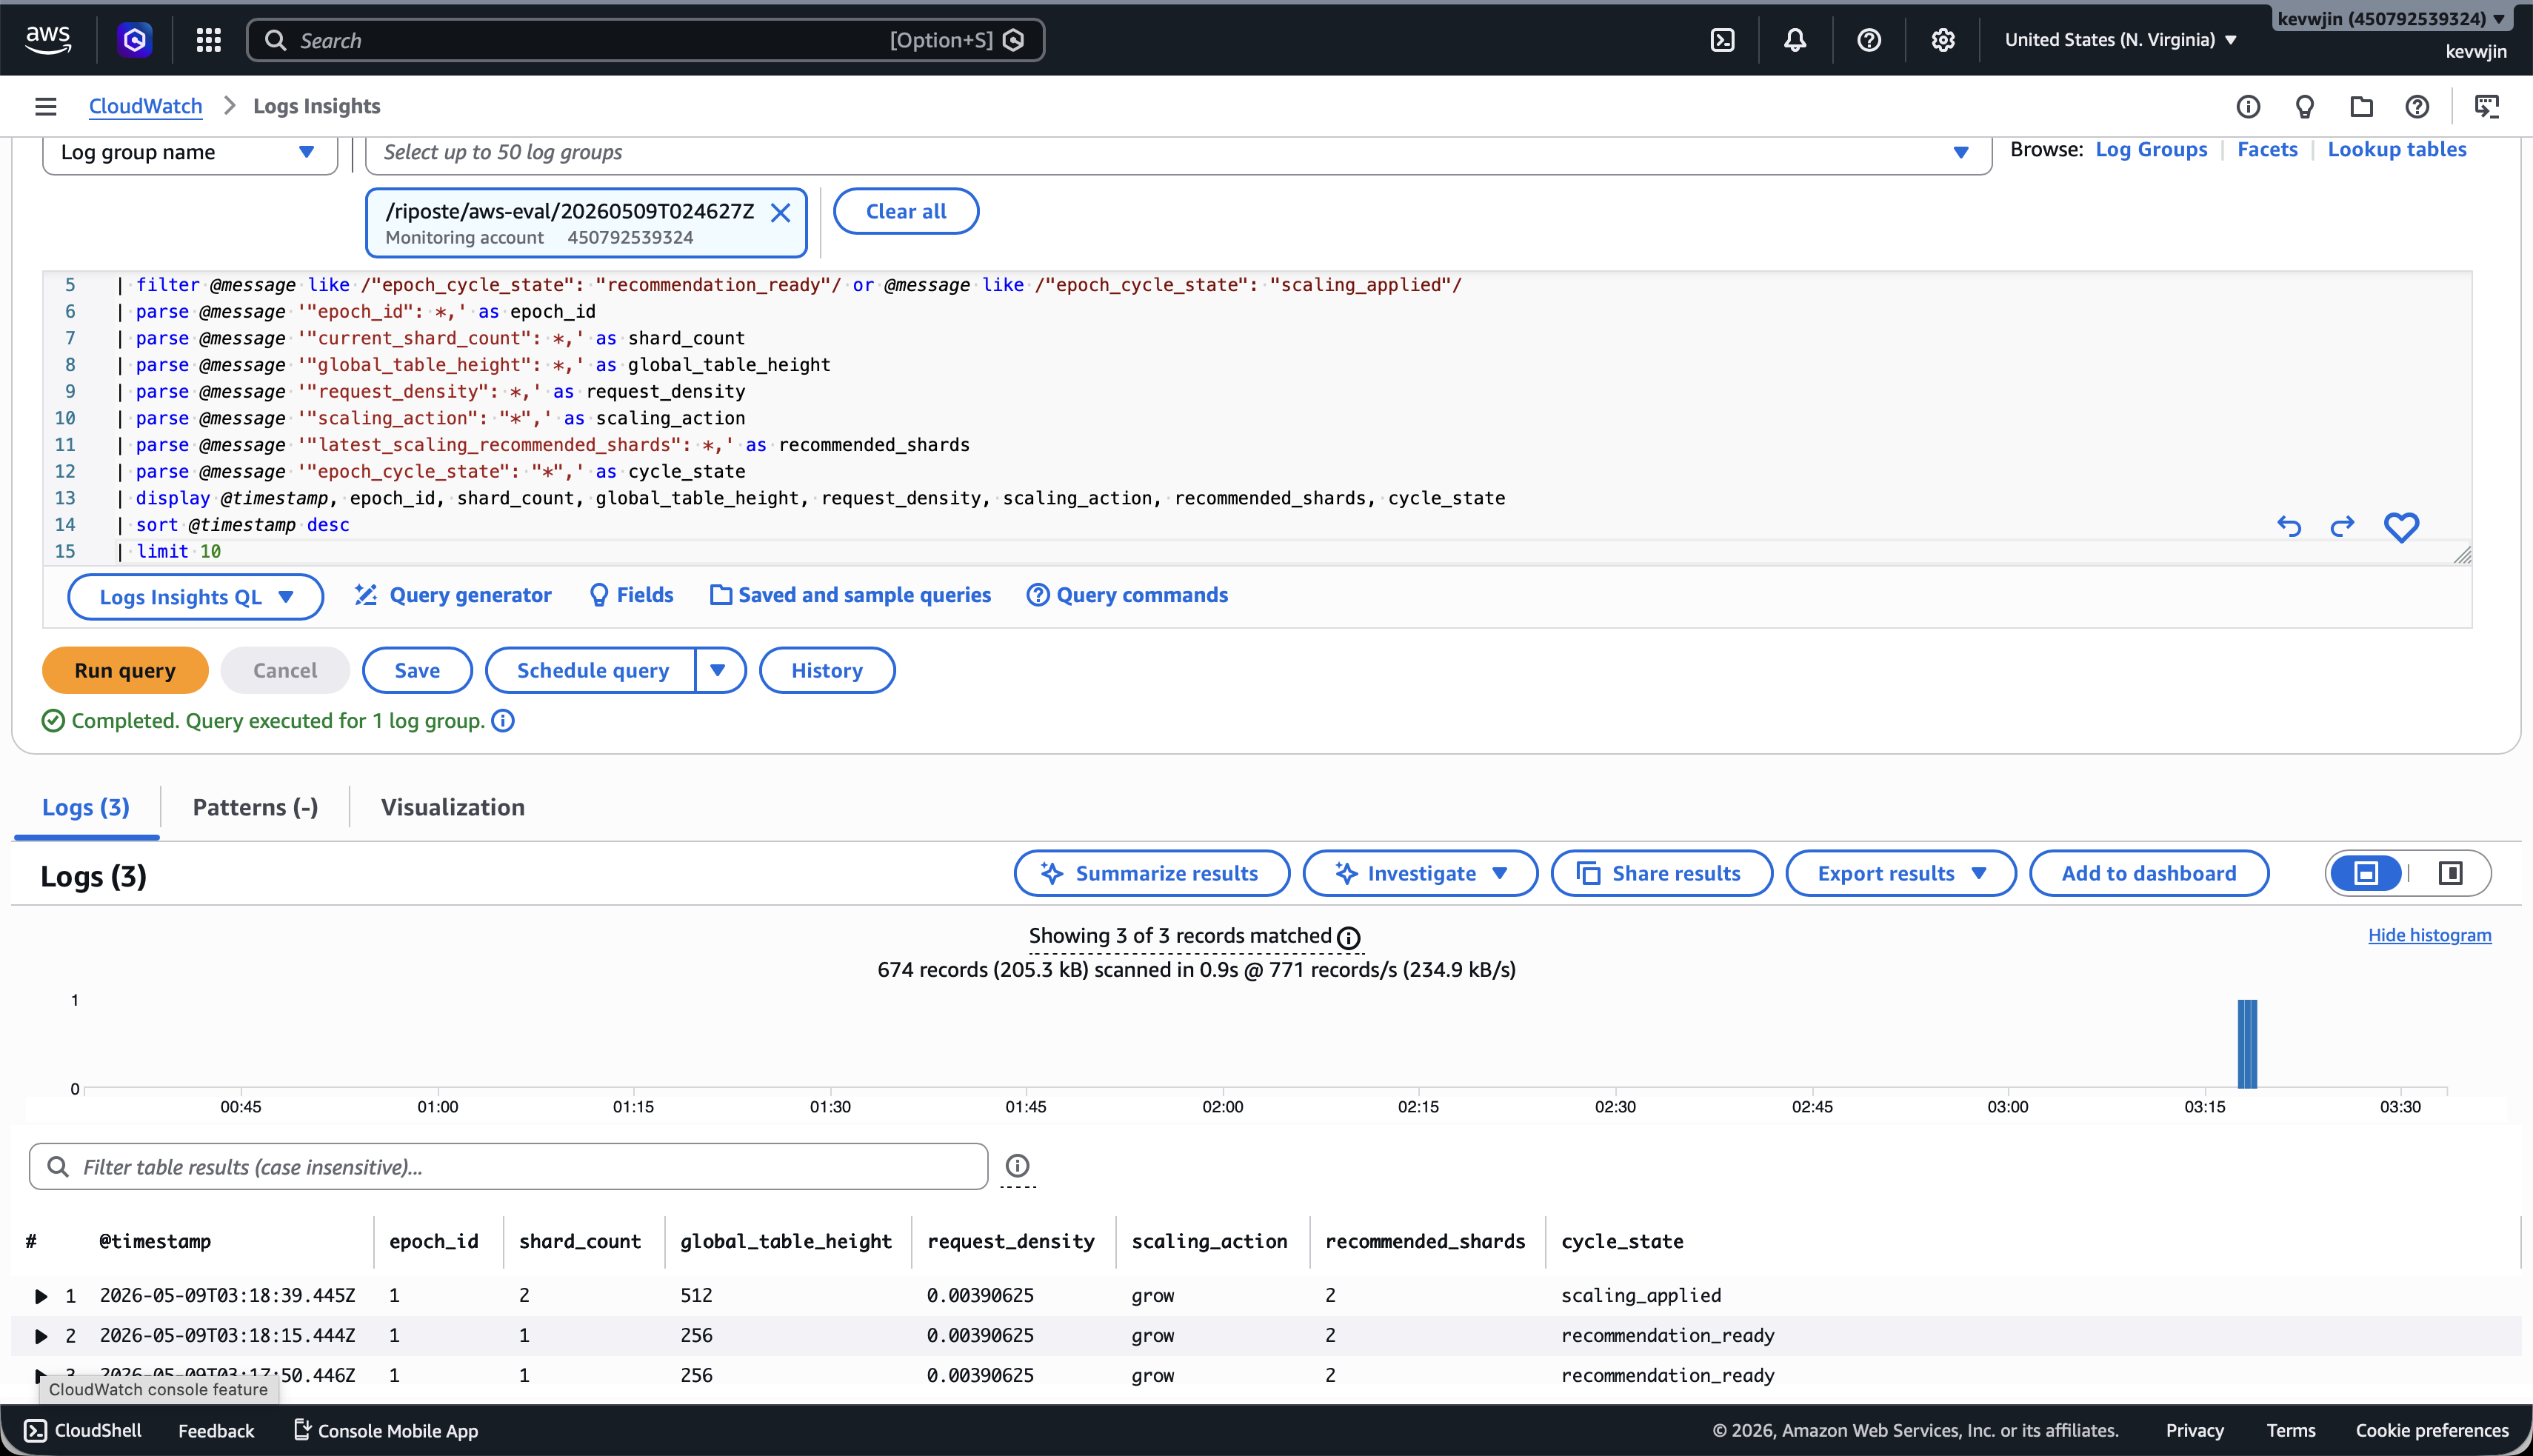
\includegraphics[width=0.95\textwidth]{figures/test-scaling-grow-applied.png}
\caption{T2 scaling evidence: request density 0.00390625 produced \texttt{grow}; applying the recommendation changed shard count from one to two and global table height from 256 to 512.}
\label{fig:test-scaling}
\end{figure*}

\subsection{T3 Failure: Hot-Standby Promotion}

The failure test stopped the active shard 0 leader and verified that the coordinator promoted the hot standby before accepting a follow-up write. Figure~\ref{fig:test-failure} shows the event sequence: the scenario started, the active shard was stopped, shard 0 was auto-promoted, and the post-promotion write reached the promoted standby. This test covers the shard availability mechanism; it does not claim that every partial in-flight client exchange survives a shard crash, because partial Upload1/Upload2 state remains a known limitation.

\begin{figure*}[!t]
\centering
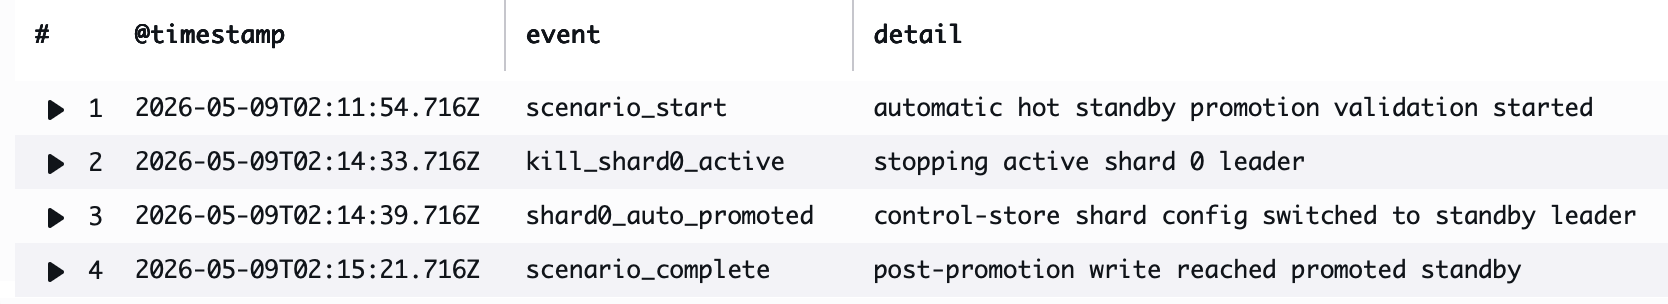
\includegraphics[width=0.95\textwidth]{figures/test-failure-auto-promotion.png}
\caption{T3 failure evidence: active shard 0 leader termination followed by hot-standby promotion and a successful post-promotion write.}
\label{fig:test-failure}
\end{figure*}

\subsection{T4 Security: Network Access Controls}

The security test inspected the EC2 security group used by the AWS evaluation. As shown in Figure~\ref{fig:test-security}, SSH ingress was restricted to the evaluator \texttt{/32} address, while application traffic was allowed from the evaluation security group. The screenshot shows no broad public application-port ingress rule. This separates operator access from internal service communication and avoids exposing the application ports to the Internet. The security group rules are not the entire security model: runtime IAM constrains AWS service access, and the RPC path uses project TLS certificates. However, this test confirms the basic network boundary enforced by the deployed AWS environment.

\begin{figure*}[!t]
\centering
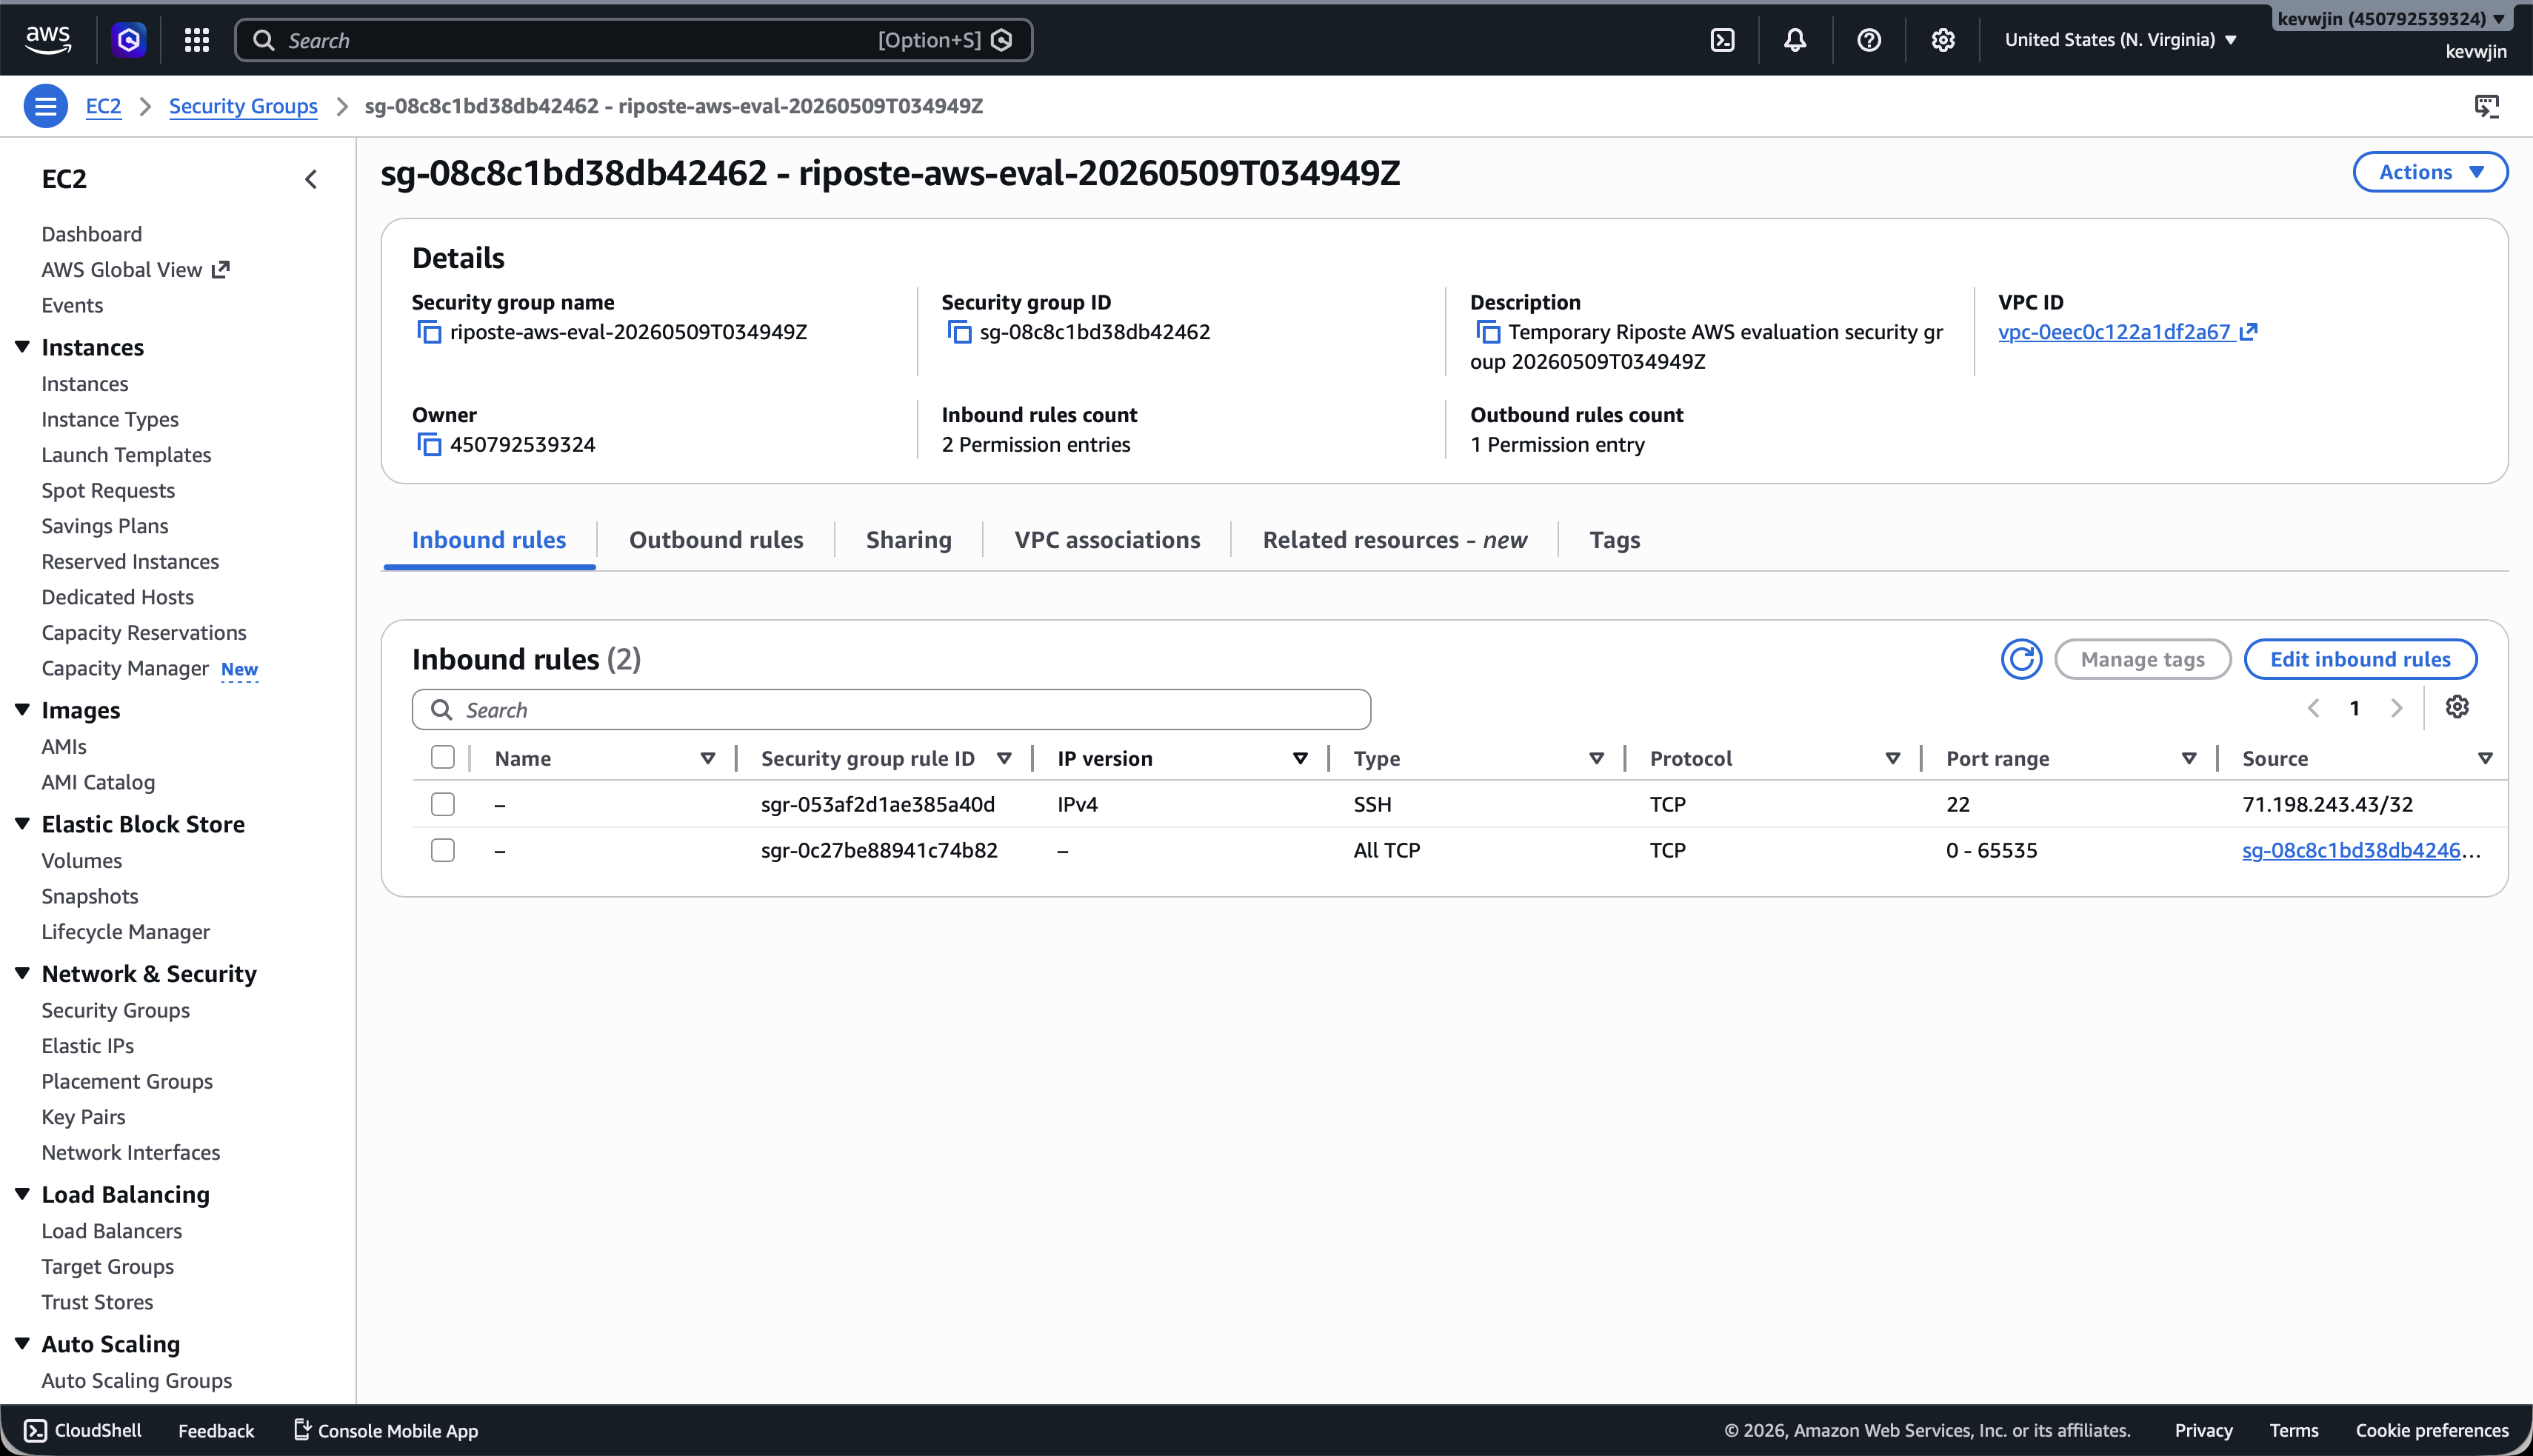
\includegraphics[width=0.95\textwidth]{figures/test-security-sg-rules.png}
\caption{T4 security evidence: EC2 security group rules restrict SSH to the evaluator IP and scope application traffic to the evaluation security group.}
\label{fig:test-security}
\end{figure*}

\subsection{T5 Performance: Accepted Upload Throughput}

The performance test is reported in Section~VI rather than as a separate CloudWatch screenshot. It follows the same methodology as the Riposte reproduction paper: accepted uploads per second under hammer load, with a same-run comparison between a direct single-shard baseline and the sharded coordinator path. The AWS run accepted 38,908 baseline uploads and 79,024 sharded uploads over the measured epoch, corresponding to a 103.10\% increase. The test result supports near-linear two-shard scaling of the online write-validation path, while retaining the important caveat that hammer-mode throughput is not a recoverability metric.

\section{Architectural Trade-Off Analysis}

\subsection{Latency Versus Availability}

The architecture favors availability and anonymity-set stability over minimum write latency. Riposte-style uploads are already latency-tolerant because writes are admitted during an epoch and become visible only after the epoch completes. The prototype leans into that model: completed uploads are durably staged through S3 and SQS after \texttt{Upload3}, and hot standby replicas can consume the same completed-upload stream so that a promoted standby is already close to the active state. This improves recovery behavior, but it adds write-path latency and service dependencies compared with a purely in-memory single-server design.

The same trade-off appears in coordinator routing. Multiple coordinators can accept upload traffic through shared DynamoDB-backed session state, but control-plane mutations remain fenced by a coordinator lease. That means clients can continue routing uploads through available coordinator processes while epoch lifecycle operations remain serialized. The cost is additional control-store checks and more careful error handling. A fully local coordinator would be faster and simpler, but it would not tolerate coordinator process failure or NLB routing across multiple coordinators as cleanly.

Shard promotion makes a similar compromise. Hot standby is faster to recover than cold replay because the standby has already processed the completed-upload stream. However, the standby path consumes compute, queue, and storage resources during normal operation. The prototype therefore improves availability by accepting extra steady-state work rather than waiting to reconstruct shard state only after failure.

\subsection{Cost Versus Elasticity}

Elasticity is deliberately bounded. The system can persist scaling recommendations and apply them between epochs, but the current implementation activates preconfigured spare shard inventory rather than provisioning new EC2 instances automatically. This keeps the evaluation controllable and avoids changing the active topology during an epoch, but it means the deployment must pay for cold spare capacity before that capacity is needed. True EC2 provisioning would reduce idle cost, but it would require a stronger orchestration layer for instance launch, health validation, queue creation, topology publication, and rollback.

This boundary is also connected to the privacy model. Each active shard is part of the anonymity set for the rows it owns. Scaling during an active epoch could split traffic mid-batch, reduce the number of writes observed by a shard, and create smaller anonymity sets for some users. Applying topology changes only between epochs preserves a stable interpretation of each batch and makes result publication easier to reason about. The trade-off is that the system cannot instantly react to traffic spikes; it can only make safe scaling decisions at epoch boundaries.

Hot standby further increases the cost of elasticity. With standby ingestion enabled, each completed upload may be processed by both active and standby replicas. For two active shards, the deployment uses four SQS queues: active and standby queues for each shard. This doubles some ingestion work, but it reduces promotion delay. The design therefore spends more on the write side to keep recovery and next-epoch scaling predictable.

\subsection{Complexity Versus Manageability}

The project chooses managed AWS services for coordination and durable work boundaries instead of implementing every distributed systems primitive directly. DynamoDB provides conditional writes for leases, fencing tokens, session records, shard topology, epoch snapshots, and scaling recommendations. SQS provides redelivery for post-\texttt{Upload3} work, and S3 stores completed-upload payloads and published artifacts. This reduces the burden of operating a custom metadata cluster, but it increases application complexity because the code must handle conditional-write failures, queue redelivery, idempotence, and cross-service observability.

The alternative would be a tighter self-managed architecture, such as a replicated coordinator built around a consensus protocol. That might simplify some application-level state transitions because the coordinator state machine would be replicated directly. However, it would move operational responsibility into the project: leader election, log compaction, membership changes, backup, monitoring, and recovery would become part of the deployed system. For this prototype, DynamoDB was a pragmatic choice because the control state is mostly key-value, low-rate, and conditional.

There is still complexity in the current design. Upload admission spans clients, coordinators, shard leaders, shard followers, DynamoDB sessions, S3 payloads, and SQS pointers. The actor-style coordinator refactor, explicit error taxonomy, shared session store, and status artifacts were added to make that complexity more manageable. The resulting system is more verbose than the original single-process path, but it is easier to test, observe, and harden because state ownership and failure boundaries are explicit.

\subsection{Consistency Implications}

The system uses different consistency models for different parts of the workload. Epoch control and shard topology are strongly serialized through the control store and coordinator fencing. Only the lease holder can mutate epoch state or apply a new shard configuration. Each epoch also records an immutable shard-config snapshot, so historical results can be interpreted using the topology that was active when the epoch ran.

Upload routing is less centralized. Coordinators behind the NLB can route uploads as long as the shared control store reports an active accepting epoch and the shared session store can recover the session. This improves availability, but it requires strict session identity checks. A bad or missing session remains a hard protocol error, while an inactive coordinator is distinguishable from a closed epoch. That distinction matters because clients should retry authority-routing failures differently from completed-epoch shutdown.

The ingestion path is at-least-once until acknowledged. A completed upload is durable after the shard writes the payload to S3 and sends the SQS pointer; workers delete the SQS message only after processing succeeds. Redelivery is expected if a worker fails before acknowledgement, so each replica records completed uploads in a DynamoDB ledger and skips duplicate work when a redelivered pointer refers to an already committed upload. This covers the demonstrated commit-before-SQS-delete ambiguity. The remaining hardening area is narrower: a crash after shard-local mutation but before the ledger commit can still require stronger ordering or local durable commit records.

Overall, the architecture separates consistency domains intentionally. Control-plane changes are fenced and serialized. Data-plane upload routing is shared and recoverable. Post-upload processing is durable and retryable. This division improves deployability, but it also means correctness depends on clear boundaries between epoch state, session state, shard-local processing, and published results.

\section{Conclusions}

This project demonstrates that a Riposte-style anonymous write relay can be adapted into a cloud-hosted, dynamically sharded architecture without abandoning the epoch-batched privacy model. The system preserves stable epoch boundaries, routes global rows across multiple shards, uses shared control and session state for multi-coordinator ingress, and moves completed-upload processing behind a durable S3/SQS boundary. The AWS evaluation showed that sharding improved measured write throughput, hot standby promotion preserved shard availability, and scaling recommendations could be applied safely between epochs.

The main lesson is that privacy-preserving architecture changes where the hard systems problems appear. Ordinary web systems often optimize for immediate request completion and elastic scaling at any time. In this system, scaling and failover must respect anonymity sets, epoch consistency, and the multi-step write protocol. As a result, the design uses epoch boundaries as the safe point for topology changes, DynamoDB as a fenced control plane, and SQS/S3 as the durable boundary after a write has been accepted.

The implementation also shows the value of managed cloud services for a prototype. DynamoDB conditional writes were well suited to leases, fencing, topology records, and session recovery. NLB separated custom TCP write ingress from individual coordinator processes, while ALB gave the stateless read path request-aware HTTP routing and semantic health checks. SQS and S3 provided durable post-upload replay without forcing large payloads into queue messages. Terraform and scripted artifact collection made the experiments repeatable enough to support quantitative reporting. At the same time, these choices introduced service coupling and operational complexity that would need production-grade monitoring, alerting, retention policies, and cost controls.

Several limitations remain. The strongest current durability boundary starts after successful \texttt{Upload3}; partial shard-side \texttt{Upload1}/\texttt{Upload2} state is not fully replayable after shard death. Scaling activates preconfigured spare shards rather than provisioning EC2 instances automatically. The performance measurements are throughput-oriented and do not include P95/P99 upload latency or complete per-instance CPU, memory, disk, and network graphs. The current prototype also assumes a centrally operated AWS deployment, even though the architecture could evolve toward independently operated shard leaders or followers.

Future work should first harden the remaining correctness boundary before the completed-upload ledger is written, especially crashes after shard-local mutation but before ledger commit. The next major step is full autoscaling: provision shard instances, validate health, create or attach queues, update topology only between epochs, and roll back safely on partial failure. Additional work should add runtime shard membership management, richer CloudWatch dashboards, stronger per-instance resource telemetry, and a cleaner read-side publication pipeline. Finally, the privacy architecture could be extended toward decentralized shard operation, where independent parties host shard replicas and cryptographic participation mechanisms help clients decide which anonymity sets or communities they are willing to use.

\begin{thebibliography}{1}

\bibitem{riposte}
H. Corrigan-Gibbs, D. Boneh, and D. Mazi\`eres, ``Riposte: An anonymous messaging system handling millions of users,'' in \emph{Proc. IEEE Symposium on Security and Privacy}, 2015. [Online]. Available: \url{https://www.scs.stanford.edu/~dm/home/papers/corrigan-gibbs:riposte-full.pdf}

\bibitem{pircompressed}
H. Corrigan-Gibbs and D. Kogan, ``Private information retrieval with compressed queries and amortized query processing,'' Microsoft Research. [Online]. Available: \url{https://www.microsoft.com/en-us/research/publication/pir-compressed-queries-amortized-computation/}

\bibitem{anysphere}
A. Lunnemark, S. Zhang, and S. Asif, ``Anysphere: Private communication in practice,'' Security Whitepaper, 2022. [Online]. Available: \url{https://anysphere-messaging.com/anysphere-whitepaper.pdf}

\bibitem{vsssimplified}
N. Chandran, V. Goyal, S. Kannan, and R. Ostrovsky, ``Verifiable secret sharing simplified,'' Cryptology ePrint Archive, Paper 2023/1196, 2023. [Online]. Available: \url{https://eprint.iacr.org/2023/1196}

\bibitem{ringreferral}
``Ring Referral: Efficient publicly verifiable ad hoc credential scheme,'' Cryptology ePrint Archive, Paper 2025/524, 2025. [Online]. Available: \url{https://eprint.iacr.org/2025/524}

\bibitem{awst3}
Amazon Web Services, ``Amazon EC2 T3 instances.'' [Online]. Available: \url{https://aws.amazon.com/ec2/instance-types/t3/}

\bibitem{awselb}
Amazon Web Services, ``Elastic Load Balancing pricing.'' [Online]. Available: \url{https://aws.amazon.com/elasticloadbalancing/pricing/}

\bibitem{awsdynamodb}
Amazon Web Services, ``Amazon DynamoDB pricing for on-demand capacity.'' [Online]. Available: \url{https://aws.amazon.com/dynamodb/pricing/on-demand/}

\bibitem{awssqs}
Amazon Web Services, ``Amazon SQS pricing.'' [Online]. Available: \url{https://aws.amazon.com/sqs/pricing/}

\bibitem{awss3}
Amazon Web Services, ``Amazon S3 pricing.'' [Online]. Available: \url{https://aws.amazon.com/s3/pricing/}

\bibitem{awscloudwatch}
Amazon Web Services, ``Amazon CloudWatch pricing.'' [Online]. Available: \url{https://aws.amazon.com/cloudwatch/pricing/}

\end{thebibliography}

\end{document}
